
\documentclass{beamer}
\usetheme{ucl}

%%% Increase the height of the banner: the argument is a scale factor >=1.0
%\setbeamertemplate{banner}[ucl][0.1]

%%% Change the colour of the main banner
%%% The background should be one of the UCL colours (except pink or white):
%%%   black,darkpurple,darkred,darkblue,darkgreen,darkbrown,richred,midred,
%%%   navyblue,midgreen,darkgrey,orange,brightblue,brightgreen,lightgrey,
%%%   lightpurple,yellow,lightblue,lightgreen,stone
\setbeamercolor{banner}{bg=darkpurple}
%\setbeamercolor{banner}{bg=yellow,fg=black}

%%% Add a stripe behind the banner
%\setbeamercolor{banner stripe}{bg=darkpurple,fg=black}

%%% The main structural elements
\setbeamercolor{structure}{fg=black}

%%% Author/Title/Date and slide number in the footline
\setbeamertemplate{footline}[author title date]

%%% Puts the section/subsection in the headline
% \setbeamertemplate{headline}[section]

%%% Puts a navigation bar on top of the banner
%%% For this to work correctly, the each \section command needs to be
%%% followed by a \subsection. Requires one extra compile.
% \setbeamertemplate{headline}[miniframes]
%%% Accepts an optional argument determining the width
% \setbeamertemplate{headline}[miniframes][0.3\paperwidth]


%%% Puts the frame title in the banner
%%% Won't work correctly with the above headline templates
%\useoutertheme{ucltitlebanner}
%%% Similar to above, but smaller (and puts subtitle on same line as title)
\useoutertheme[small]{ucltitlebanner}

%%% Gives block elements (theorems, examples) a border
% \useinnertheme{blockborder}
%%% Sets the body of block elements to be clear
% \setbeamercolor{block body}{bg=white,fg=black}

%%% Include CSML logo on title slide
%\titlegraphic{\includegraphics[width=0.16\paperwidth]{csml_logo}}

%%% Include CSML logo in bottom right corner of all slides
%\logo{\includegraphics[width=0.12\paperwidth]{csml_logo}}

%%% Set a background colour
% \setbeamercolor{background canvas}{bg=lightgrey}

%%% Set a background image
%%% Some sample images are available from the UCL image store:
%%%   https://www.imagestore.ucl.ac.uk/home/start
% \setbeamertemplate{background canvas}{%
%   \includegraphics[width=\paperwidth]{imagename}}



%%%%%% Some other settings that can make things look nicer
%%% Set a smaller indent for description environment
\setbeamersize{description width=2em}
%%% Remove nav symbols (and shift any logo down to corner)
\setbeamertemplate{navigation symbols}{\vspace{-2ex}}








\DeclareMathOperator{\Cov}{Cov}
\DeclareMathOperator{\Var}{Var}
\DeclareMathOperator{\E}{\mathbb{E}}
\DeclareMathOperator{\Proba}{\mathbb{P}}

\newcommand{\Covb}[2]{\ensuremath{\Cov\!\left[#1,#2\right]}}
\newcommand{\Eb}[1]{\ensuremath{\E\!\left[#1\right]}}
\newcommand{\Pb}[1]{\ensuremath{\Proba\!\left[#1\right]}}
\newcommand{\Varb}[1]{\ensuremath{\Var\!\left[#1\right]}}

% norm
\newcommand{\norm}[1]{\| #1 \|}

\newcommand{\indep}{\rotatebox[origin=c]{90}{$\models$}}





\usepackage{mathptmx,amsmath,amssymb,graphicx,bibentry,bbm,ragged2e}
\usepackage[english]{babel}

\makeatletter

\newcommand{\noun}[1]{\textsc{#1}}
\newcommand{\jitem}[1]{\item \begin{justify} #1 \end{justify} \vfill{}}
\newcommand{\sframe}[2]{\frame{\frametitle{#1} #2}}

\newenvironment{centercolumns}{\begin{columns}[c]}{\end{columns}}
%\newenvironment{jitem}{\begin{justify}\begin{itemize}}{\end{itemize}\end{justify}}



%\usetheme{Warsaw}
%\setbeamertemplate{footline}[text line]{}
%\setbeamertemplate{headline}{}
%\setbeamercolor{structure}{fg=purple!50!blue, bg=purple!50!blue}

%\setbeamersize{text margin left=15pt,text margin right=15pt}

%\setbeamercovered{transparent}


\@ifundefined{showcaptionsetup}{}{%
 \PassOptionsToPackage{caption=false}{subfig}}
\usepackage{subfig}

\usepackage[utf8]{inputenc}
\usepackage[T1]{fontenc}

\usepackage{multirow}


\makeatother

\def \draft {1}

\usepackage{xparse}
\usepackage{ifthen}
\DeclareDocumentCommand{\comment}{m o o o o}
{\ifthenelse{\draft=1}{
    \textcolor{red}{\textbf{C : }#1}
    \IfValueT{#2}{\textcolor{blue}{\textbf{A1 : }#2}}
    \IfValueT{#3}{\textcolor{ForestGreen}{\textbf{A2 : }#3}}
    \IfValueT{#4}{\textcolor{red!50!blue}{\textbf{A3 : }#4}}
    \IfValueT{#5}{\textcolor{Aquamarine}{\textbf{A4 : }#5}}
 }{}
}
\newcommand{\todo}[1]{
\ifthenelse{\draft=1}{\textcolor{red!50!blue}{\textbf{TODO : \textit{#1}}}}{}
}




\begin{document}

\title[Multiscale urban growth]{A multi-scalar model for system of cities}
\author[Raimbault]{J.~Raimbault$^{1,2,3\ast}$\\\medskip
$^{\ast}$\texttt{j.raimbault@ucl.ac.uk}
}

\institute[UCL]{$^{1}$CASA, UCL\\
$^{2}$UPS CNRS 3611 Complex Systems Institute Paris\\
$^{3}$UMR CNRS 8504 G{\'e}ographie-cit{\'e}s
}


\date[1st October 2019]{CCS 2019\\
Urban Complexity\\
October 1st 2019
}

\frame{\maketitle}



% keywords Systems of cities Multi-scalar model Spatial interaction Reaction-diffusion


\section{Introduction}



\sframe{Modeling urban growth}{

%The modeling of urban growth is a crucial issue for the design of sustainable territorial policies, through the understanding of past urbanization processes and the forecasting of future urban trajectories.

% Q : integrate macro indics ? bof, not used the more elaborated ones

% striking image intro

% history of Singapore: emerged within a multi-scale context - and then local growth (strongly shaped by its interactions at many scales)


}


\sframe{Growth models at the mesoscopic scale}{

%Several models have been proposed at different scales and integrating different dimensions of urban systems, such as land-use transport interaction models \cite{wegener2004land} 
%At the scale of a metropolitan area, Land-use Transport Interaction models \cite{wegener2004land} are for example a privileged tool to anticipate the answer of spatial distributions of activities (mostly residential location and economic activities) to an evolution of the accessibility landscape permitted by new transportation infrastructures. At the same scale, cellular automata models of urban growth or land-use change study more generally land-use transitions with a high spatial resolution, and are mostly data-driven \cite{clarke2007decade}.

\begin{columns}
	\begin{column}{0.5\linewidth}
		
		% includegraphics 
		
		% Nedum model ?
		
		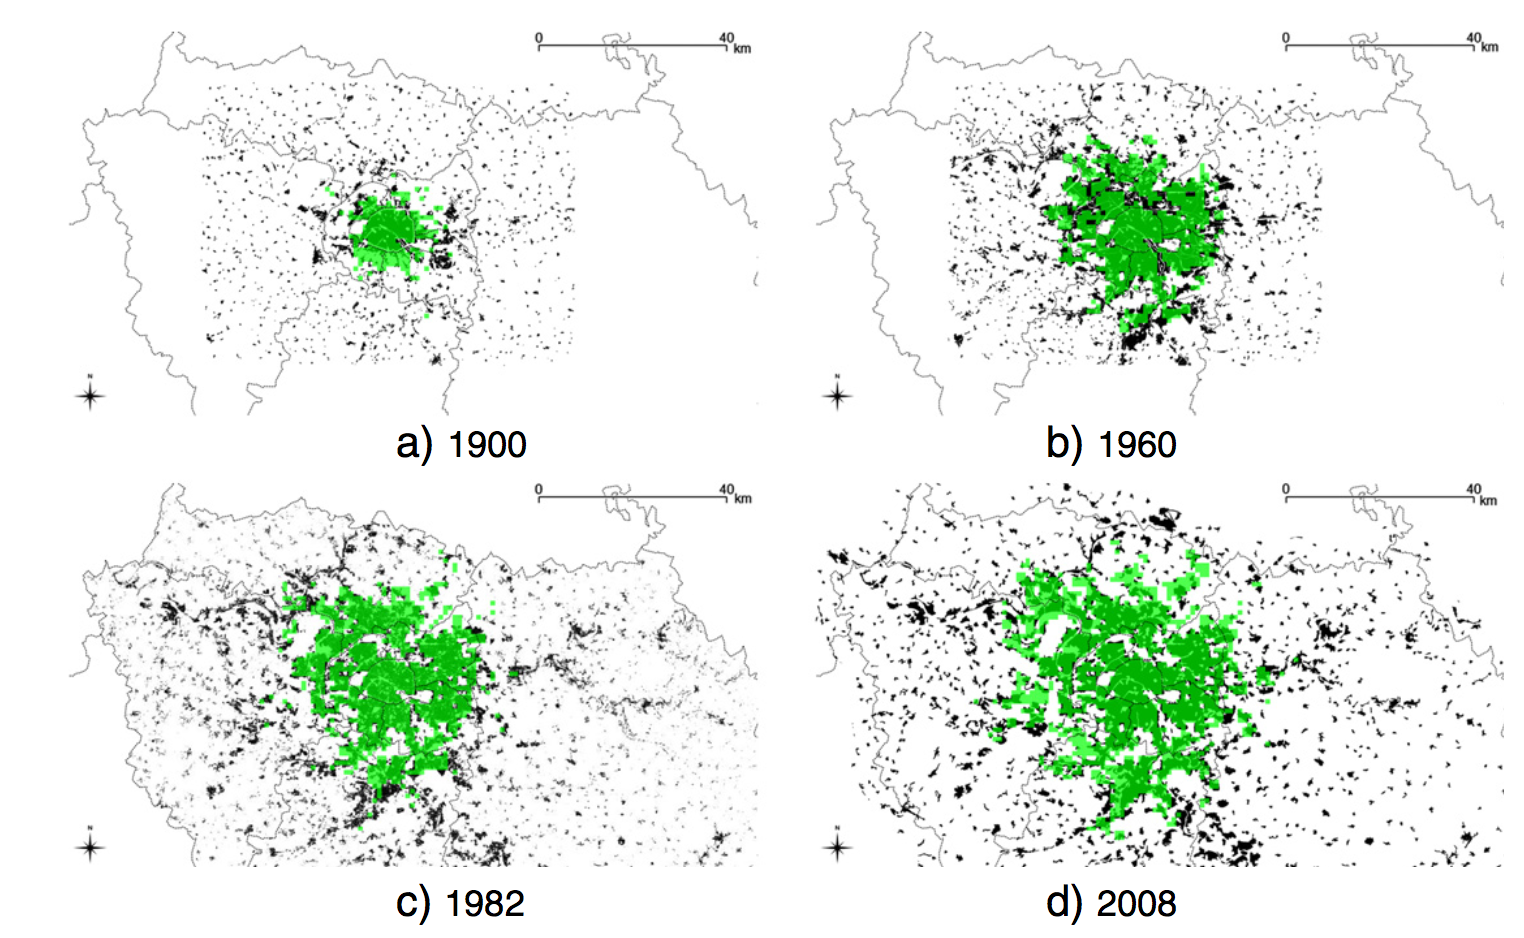
\includegraphics[width=\linewidth]{figures/nedum.png}
		
		\medskip
	
		\textit{Land-use transport models}
		
		\cite{viguie2014downscaling}
			
	\end{column}
	\begin{column}{0.5\linewidth}
		
		
		\begin{center}
	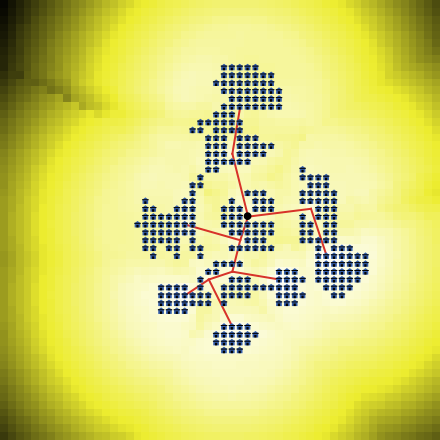
\includegraphics[width=0.85\textwidth]{figures/intro_RBD_lattice.png}
	\end{center}
	
	%\footnotesize
\textit{Hybrid urban morphogenesis model}
	
	\cite{raimbault2014hybrid}
 
 %Raimbault, J., Banos, A., \& Doursat, R. (2014, June). A Hybrid Network/Grid Model of Urban Morphogenesis and Optimization. In 4th International Conference on Complex Systems and Applications (pp. 51-60).
		
	
	\end{column}
\end{columns}




}


\sframe{Interaction models for systems of cities}{

% or systems of cities models \cite{pumain2017urban}.
% At the smaller scale of the system of cities, macroscopic models of urban growth have focused on reproducing the distribution of city sizes, either through economic processes as e.g. \cite{gabaix1999zipf}, or from a geographical point of view focusing on interactions between cities \cite{favaro2011gibrat}.


\begin{center}
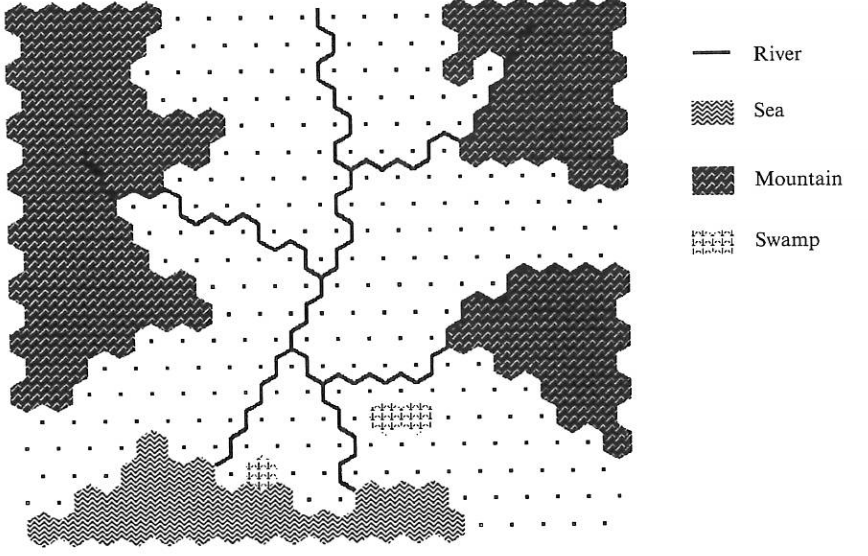
\includegraphics[width=0.55\textwidth]{figures/simpop1.png}
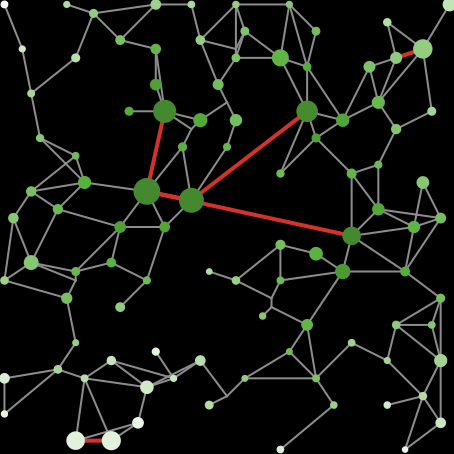
\includegraphics[width=0.42\textwidth]{figures/setup_synth_1_tick100.png}
\end{center}

\medskip

\textit{The series of Simpop models: from Simpop1 \cite{sanders1997simpop} to SimpopNet \cite{schmitt2014modelisation}}


}


\sframe{Towards multi-scalar models}{

%While multi-scalar models are recognized as crucial for the study of such systems \cite{Rozenblat2018}, they remain in practice unexplored.
%Territorial dynamics, and more particularly urban dynamics, have according to \cite{pumain1997pour} an intrinsic multi-scalar nature, with successive autonomous levels of emergence from individual microscopic agents to the mesoscopic scale of the city and the macroscopic scale of the system of cities. Furthermore, the need for sustainable territorial policies would imply the construction of multi-scalar models to take into account issues associated to each relevant scale \cite{Rozenblat2018}.

% images scales Denise


\begin{center}
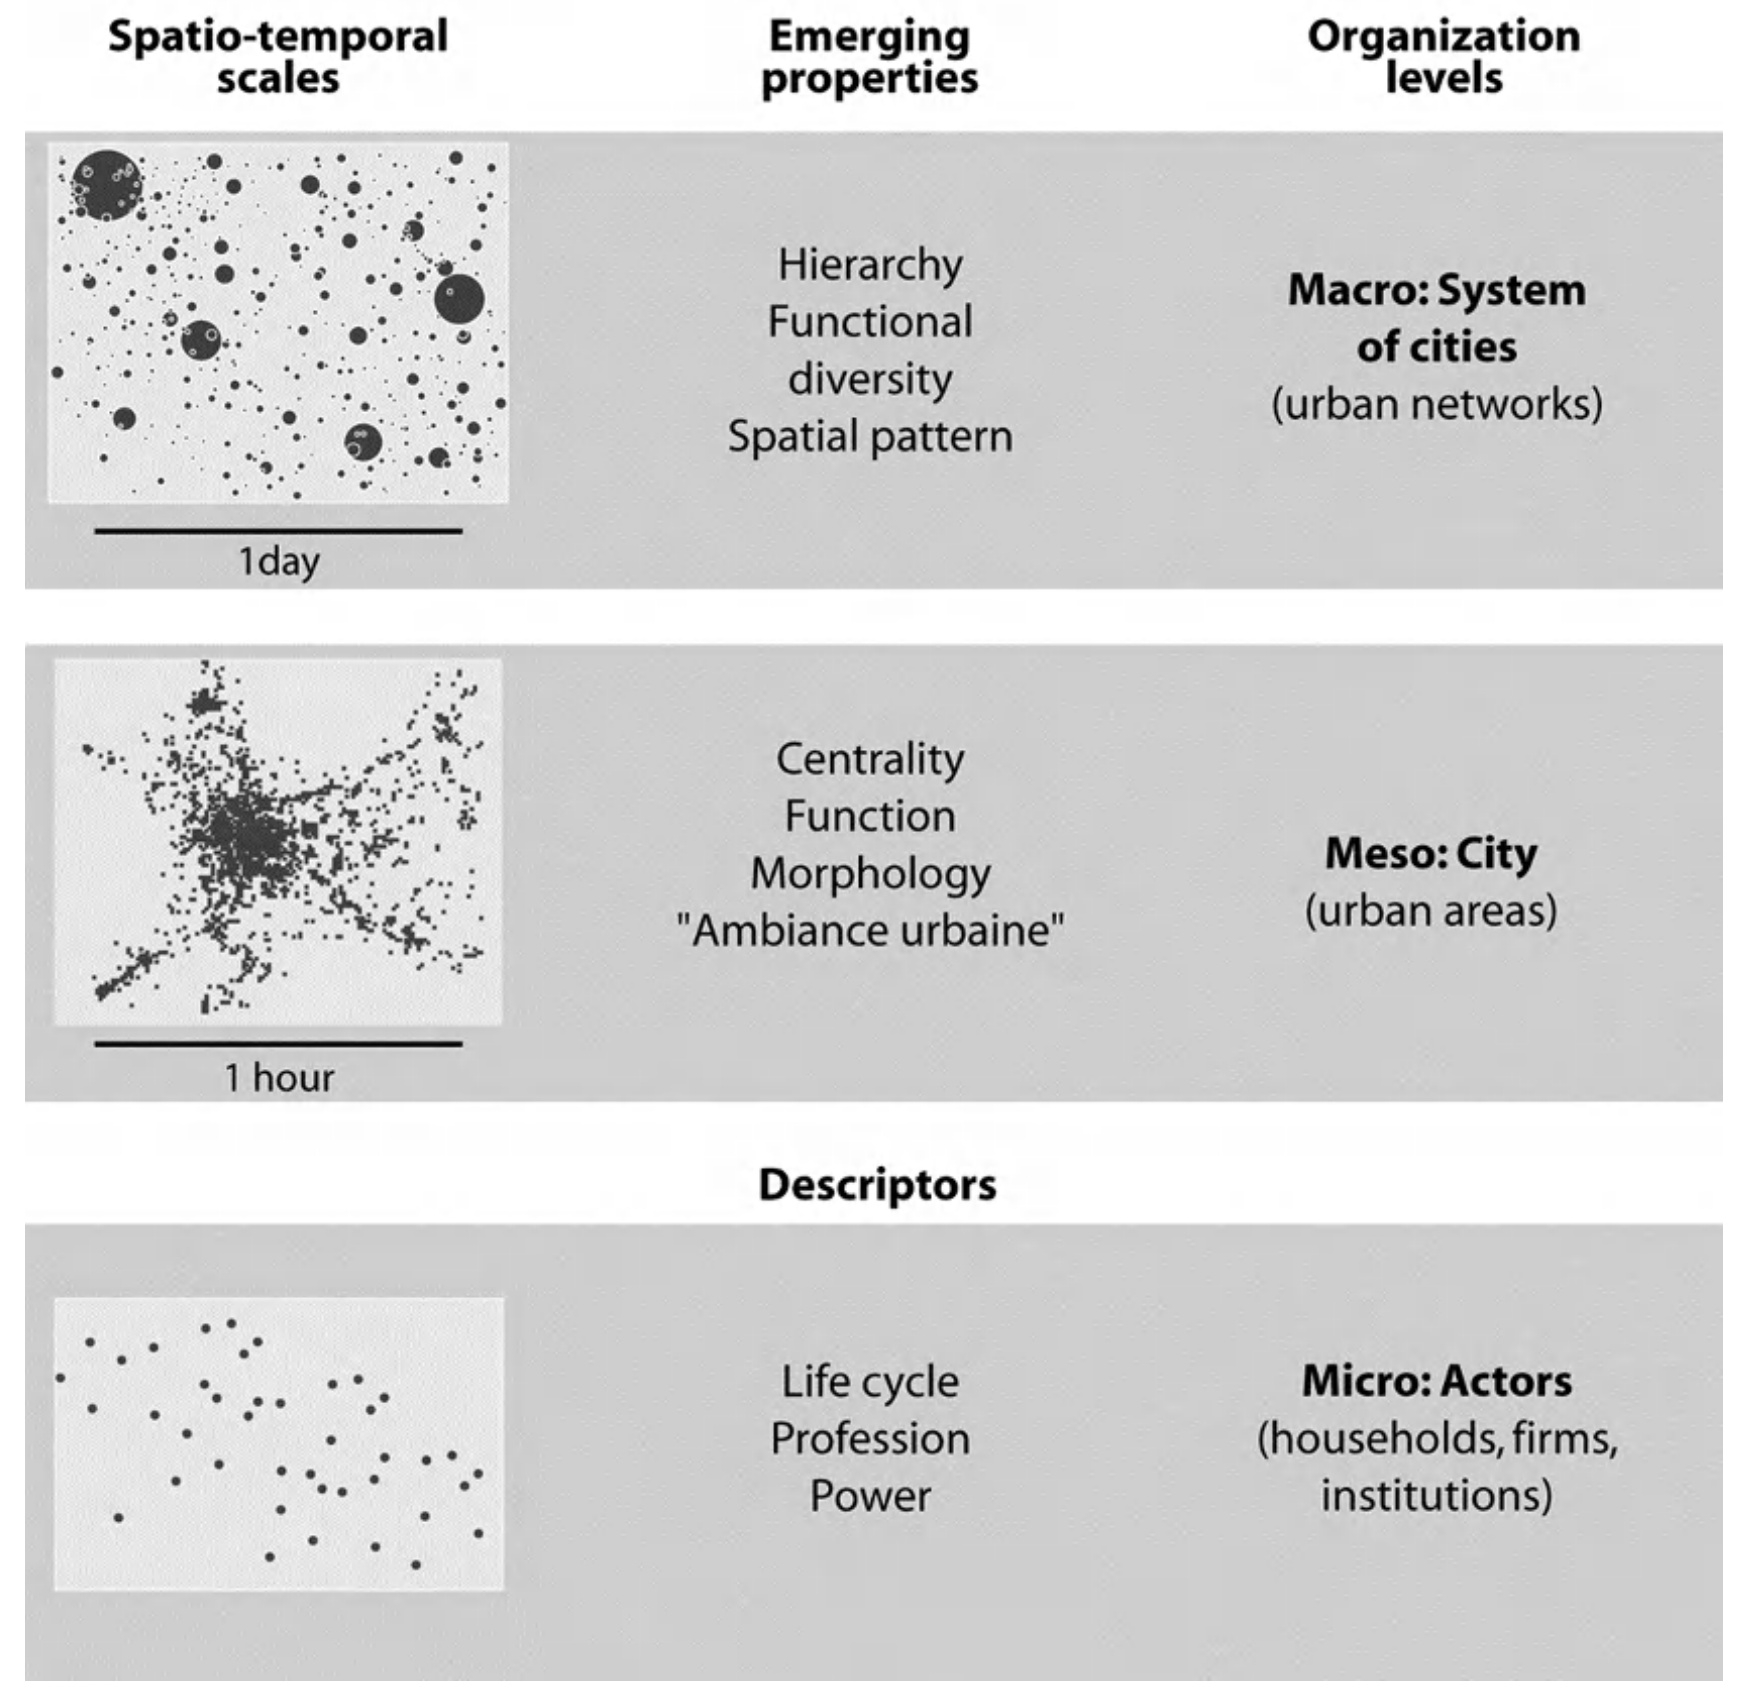
\includegraphics[height=0.65\textheight]{figures/evoltheory_scales}
\end{center}

\textit{Scales of urban systems of systems described by the evolutionary urban theory} \cite{pumain2018evolutionary}

%\textit{Systems of cities as co-evolutive systems in which interactions are crucial}
%\cite{pumain1997pour}
%\cite{pumain2008socio}
%\cite{pumain2018evolutionary}


}



\sframe{Strong coupling and multi-scalarity}{

% on model coupling: example diagram Mike flooding

\justify

$\rightarrow$ Weak inter-scale coupling, such as progressive resolution for land-use model, does not considers emergence and autonomous scales

\bigskip

$\rightarrow$ An integrated model, or strongly coupled, would be \textit{a new model extending the two coupled models in the sense that it includes them in some parameter settings or limit conditions}

\bigskip

\textbf{\textit{Urban multi-scalar complexity must be capture by a strongly coupled model}}

}


 







\sframe{Research objective}{


%This contribution contributes to that open question by introducing a multi-scale model of urban growth which focuses on the spatial structure of processes rather than on their multi-dimensionality. Therefore, we take into account only population variables, but both at the macroscopic scale of the system of cities in the legacy of \cite{pumain2017urban} and at the mesoscopic scale of the metropolitan area with an urban morphogenesis model. The coupling of these scales is a crucial novel feature of our model. We describe in the following stylized facts justifying the approach, describe the model, and summarize preliminary results from its exploration and calibration.
%This contribution introduces a parsimonious multi-scalar model for systems of cities, based on simple dimensions (mainly populations) with stylized processes, but yielding an effective strong coupling between the metropolitan mesoscopic scale and the macroscopic scale of the system of cities.

$\rightarrow$ no strongly coupled multi-scalar model in the literature

\medskip

$\rightarrow$ need to however consider ``simple'' models to be able to understand their behavior and extract knowledge from them


\bigskip
\bigskip

\textbf{Research objective: }

\medskip

\textit{Investigate a strong coupling of a simple urban system interaction network at the macroscopic scale with an urban morphogenesis model at the mesoscopic scale}


}



\section{Model description}


\sframe{Model rationale}{

\centering

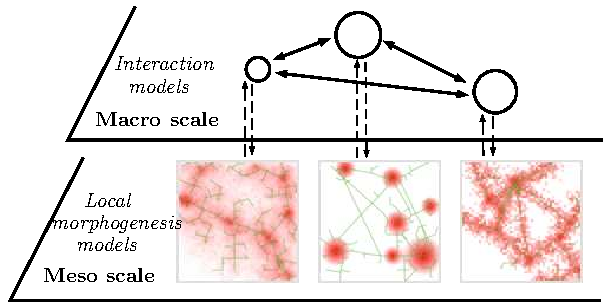
\includegraphics{figures/multiscale_morph.pdf}

}



\sframe{Model rationale}{

%The model couples the spatial interaction model of \cite{raimbault2018indirect} for the macro scale with the reaction-diffusion model for urban form studied by \cite{raimbault2018calibration}. More precisely, urban areas viewed as a population grid are embedded into the macroscopic interaction model. To evolve populations and local urban forms, one time step consists of (i) population differences are computed by the interaction model; (ii) top-down feedback modifies parameters of mesoscopic models, given control parameters to capture typical scenarios (transit-oriented development or sprawl for diffusion, metropolization or uniformization for aggregation); (iii) local urban form are evolved with the reaction-diffusion models at a given speed conditionally to the population variations; (iv) changes in urban form influence macroscopic interaction ranges (capturing the impact of local activity on global insertion), by integrating gravity flows in the area with a squared cost function making a compromise between congestion and flows.

\textbf{Model scales and objects: }

\begin{itemize}
	\item Cities as agents at the macroscopic scale
	\item Cities as population density grids at the mesoscopic scale
\end{itemize}

\medskip

\textbf{Processes: }

\begin{itemize}
	\item Interaction flows between cities and endogenous growth
	\item Urban sprawl and aggregation within urban areas
	\item \textbf{Downward feedback} Adaptation of urban form parameters to population and accessibility growth (``policy response'')
	\item \textbf{Upward feedback} Adaptation of city interaction range depending on internal performance (congested flows)
\end{itemize}


}



\sframe{Model formalization}{

At each time step:

\medskip

\begin{enumerate}
	\item Macroscopic population are evolved with the interaction model
	\item Population and accessibility differences modify the mesoscopic parameter of diffusion (sprawl) and aggregation (metropolization) \textbf{\textit{(downward feedback)}}
	\item Urban forms are evolved for each city at the mesoscopic scale to match population increases
	\item City interaction ranges are modified according to the internal performance of each city (congested flows) \textbf{\textit{(upward feedback)}}
\end{enumerate}


}


\sframe{Macroscopic model}{

% rq : does the macro mmodel captures many rank clock inversions ? kind of given variations of the rank correlation (cite macrocoevol)

% + detail indicators here

\justify

\textit{System of cities interaction model including network evolution; production of multiple co-evolution regimes and calibration for France.} 

\cite{raimbault2018indirect}

\medskip

\begin{center}
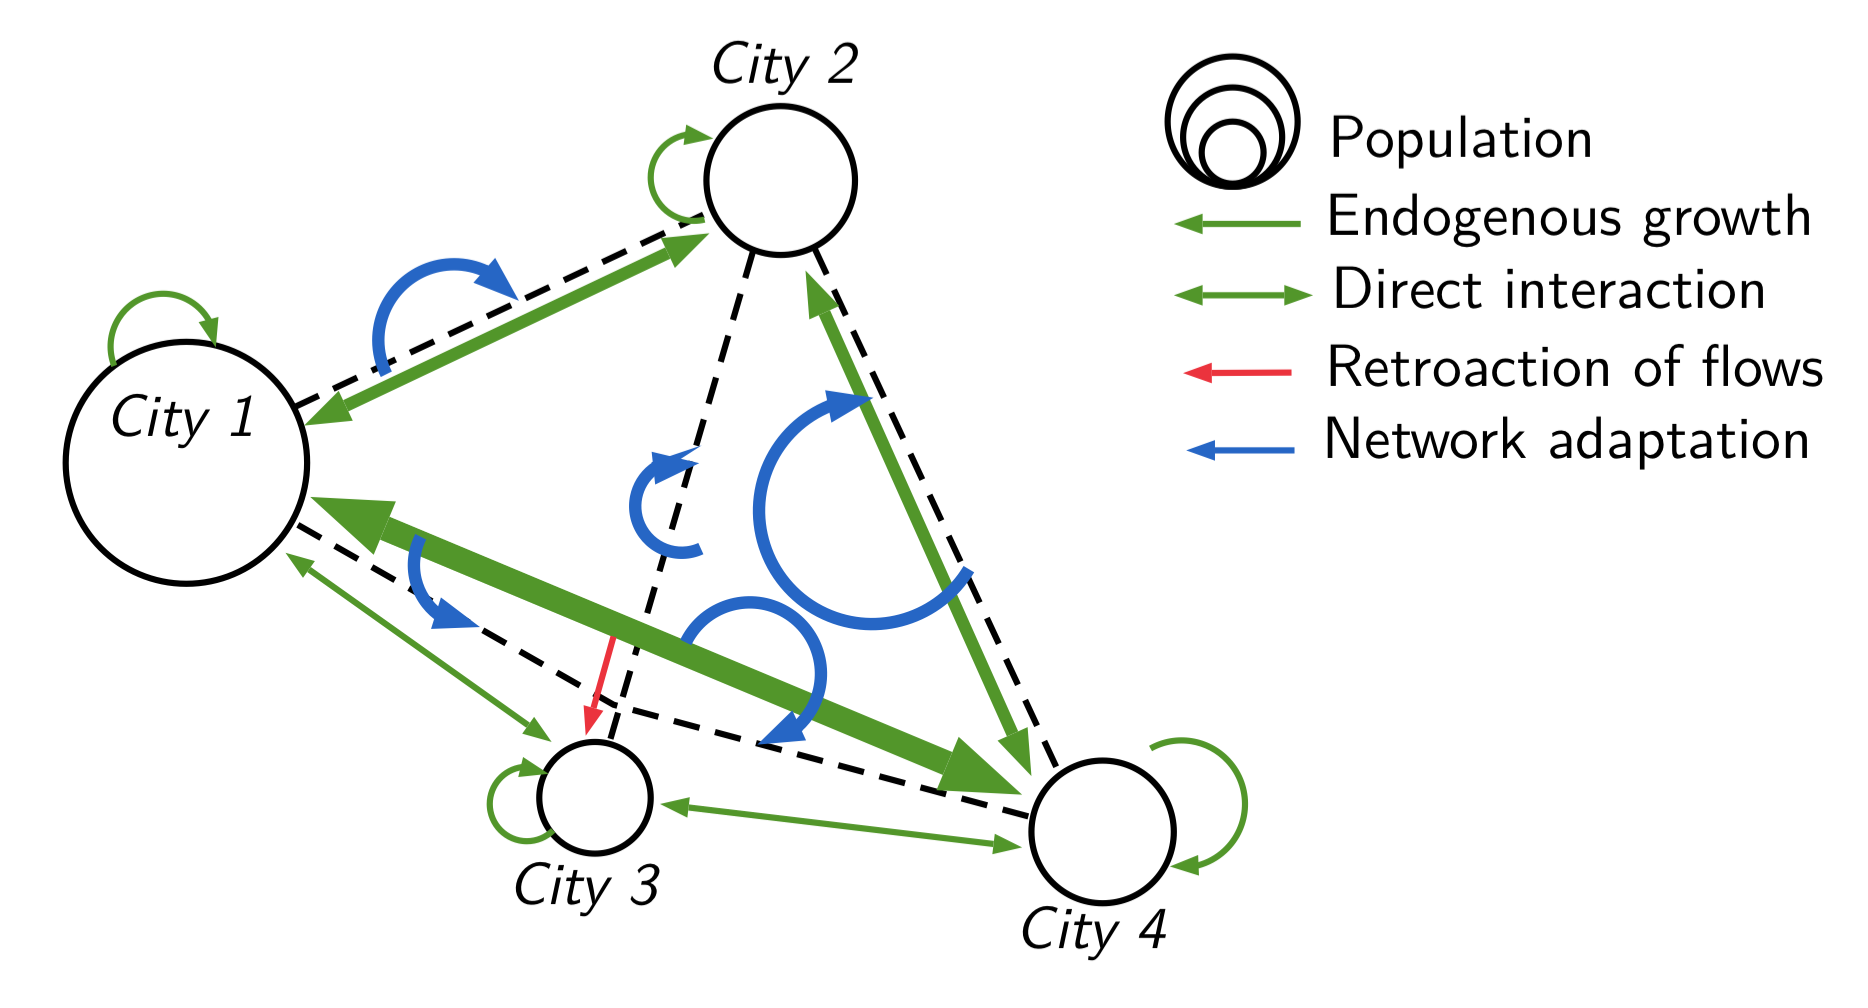
\includegraphics[width=0.72\textwidth]{figures/macrocoevol_en.png}
\end{center}

%\nocite{raimbault2019modeling}


%\bigskip
%\tiny

%Raimbault, J. (2018). Indirect evidence of network effects in a system of cities. Environment and Planning B: Urban Analytics and City Science, 2399808318774335.

%\smallskip

%Raimbault, J. (2019). Modeling the co-evolution of cities and networks. In Niel, Z., Rozenblat, C., eds. \textit{Handbook of Cities and Networks}, Edwar Elgar Publishing, \textit{in press}.

\footnotesize
\textit{Indicators at the macroscopic scale: distributions of population, accessibilities, centralities (summarized by average, hierarchy, entropy)}


}


\sframe{Mesoscopic model}{

% + detail urban form indicators


\textit{Aggregation-diffusion model at the mescoscopic scale, covering most existing urban forms in Europe} \cite{raimbault2018calibration}

\medskip

\begin{center}
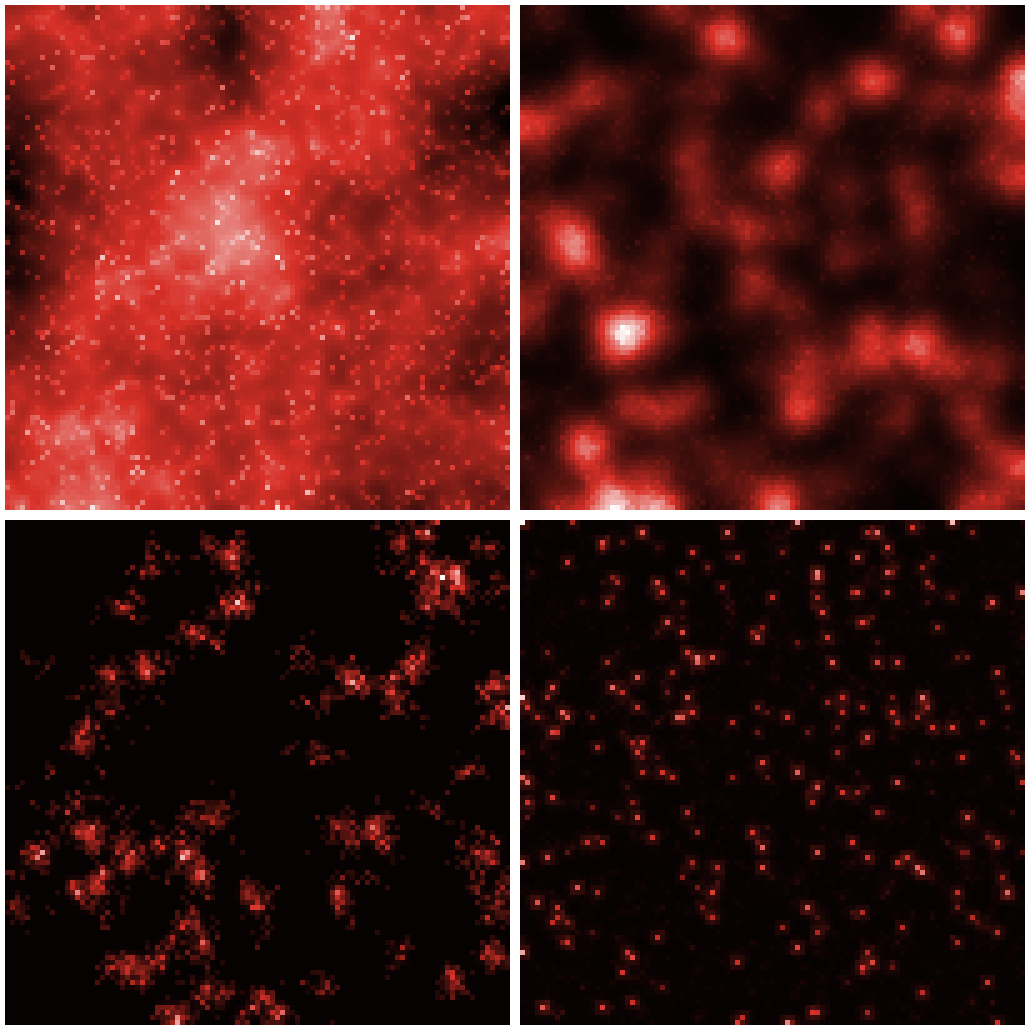
\includegraphics[height=0.6\textheight]{figures/density_Fig2}
\end{center}

%\footnotesize\textit{Examples of generated territorial shapes}

\footnotesize 
\textit{Indicators at the mesoscopic scale: urban form captured by Moran index, average distance, hierarchy, entropy}

}



\sframe{Model parameters}{

\centering


		\begin{tabular}{|c|c|c|c|}
	\hline %\tiny
		Type & Parameter & Process & Range \\\hline
		\multirow{4}{*}{Macro} & $g_i \textrm{ = } g_0$ & Endogenous growth & $\left[0 ; 0.05 \right]$ \\
		& $w_i \textrm{ = } w_G$ & Interactions weight & $\left[0 ; 0.01 \right]$  \\
		& $\gamma_i \textrm{ = } \gamma_G$ & Interactions hierarchy & $\left[0 ; 5 \right]$  \\
		& $d_i$ & Interactions decay & $\left[0 ; 1000 \right]$  \\ \hline
		\multirow{4}{*}{Meso} & $\alpha_i$ & Aggregation & $\left[0 ; 5 \right]$  \\
		& $\beta_i$ & Diffusion & $\left[0 ; 0.1 \right]$  \\
		& $t_m$ & Urban growth speed & $\{1 ; 20 \}$  \\
		& $n_d$ & Diffusion steps &  $\left[1 ; 5 \right]$ \\ \hline
		\multirow{4}{*}{Multiscale} & $\delta\alpha$ & Metropolization (downward) & $\left[-0.2 ; 0.2 \right]$  \\
		& $\delta\beta$ & Sprawl (downward) & $\left[-0.2 ; 0.2 \right]$ \\
		& $\delta d$ & Efficiency (upward) &$\left[-0.2 ; 0.2 \right]$ \\
		& $\lambda$ & Congestion cost (upward) & $\left[0 ; 10 \right]$ \\\hline
	\end{tabular}

}



\section{Results}


\sframe{Implementation}{

% Parameter space is explored with the OpenMOLE model exploration software \cite{reuillon2013openmole}, eased by the implementation of the model in scala \cite{model}.

% + pub openmole

%\footnotesize
\justify

\textit{Performance constraints: simulate $N$ mesoscopic morphogenesis models in parallel (macroscopic interactions are efficient as based on matrices)}

\medskip

$\rightarrow$ model implemented in \texttt{scala} and integrated within a broader library (including implementations of \cite{raimbault2018indirect} \cite{raimbault2018calibration}

\cite{favaro2011gibrat} \cite{cottineau2015modular})

\bigskip

\textit{Large number of parameters and output indicators}

\medskip

$\rightarrow$ integration into the OpenMOLE model exploration open source software \cite{reuillon2013openmole}

\begin{center}

\includegraphics[height=0.13\textheight]{figures/iconOM.png}

\includegraphics[height=0.13\textheight]{figures/openmole.png}
\end{center}

%(X year of computation for the results presented here)

\footnotesize
\textit{Enables seamlessly (i) model embedding; (ii) access to HPC resources; (iii) exploration and optimization algorithms}

\medskip

\textbf{Come to the satellite \textit{New Methods and Epistemologies to Explore Simulation Models} tomorrow afternoon in LHN-TR+05}

}


\sframe{Synthetic configuration}{

% The model is applied on synthetic systems of cities typical of a continental range (500km, hierarchy around 1, 20 cities), with initial local population grid configurations as monocentric.

Model applied on synthetic systems of cities:

\medskip

\begin{itemize}
	\item random positions and rank-size hierarchy ($\alpha \textrm{ = } 1.0$ and $P_0 \textrm{ = } 100,000$)
	\item countrywide urban system scale: 500km and 20 cities
	\item initial population grids as monocentric (grid of size 50 and center cell density 1000 units)
	\item simulated for 20 macroscopic time steps (order of magnitude of half a century)
\end{itemize}



}



\sframe{Statistical consistency}{

% one factor sampling

%(min around 1 for 3 indicators, above 5 for 2 and around 0.5 for 2)}

\medskip

\begin{center}
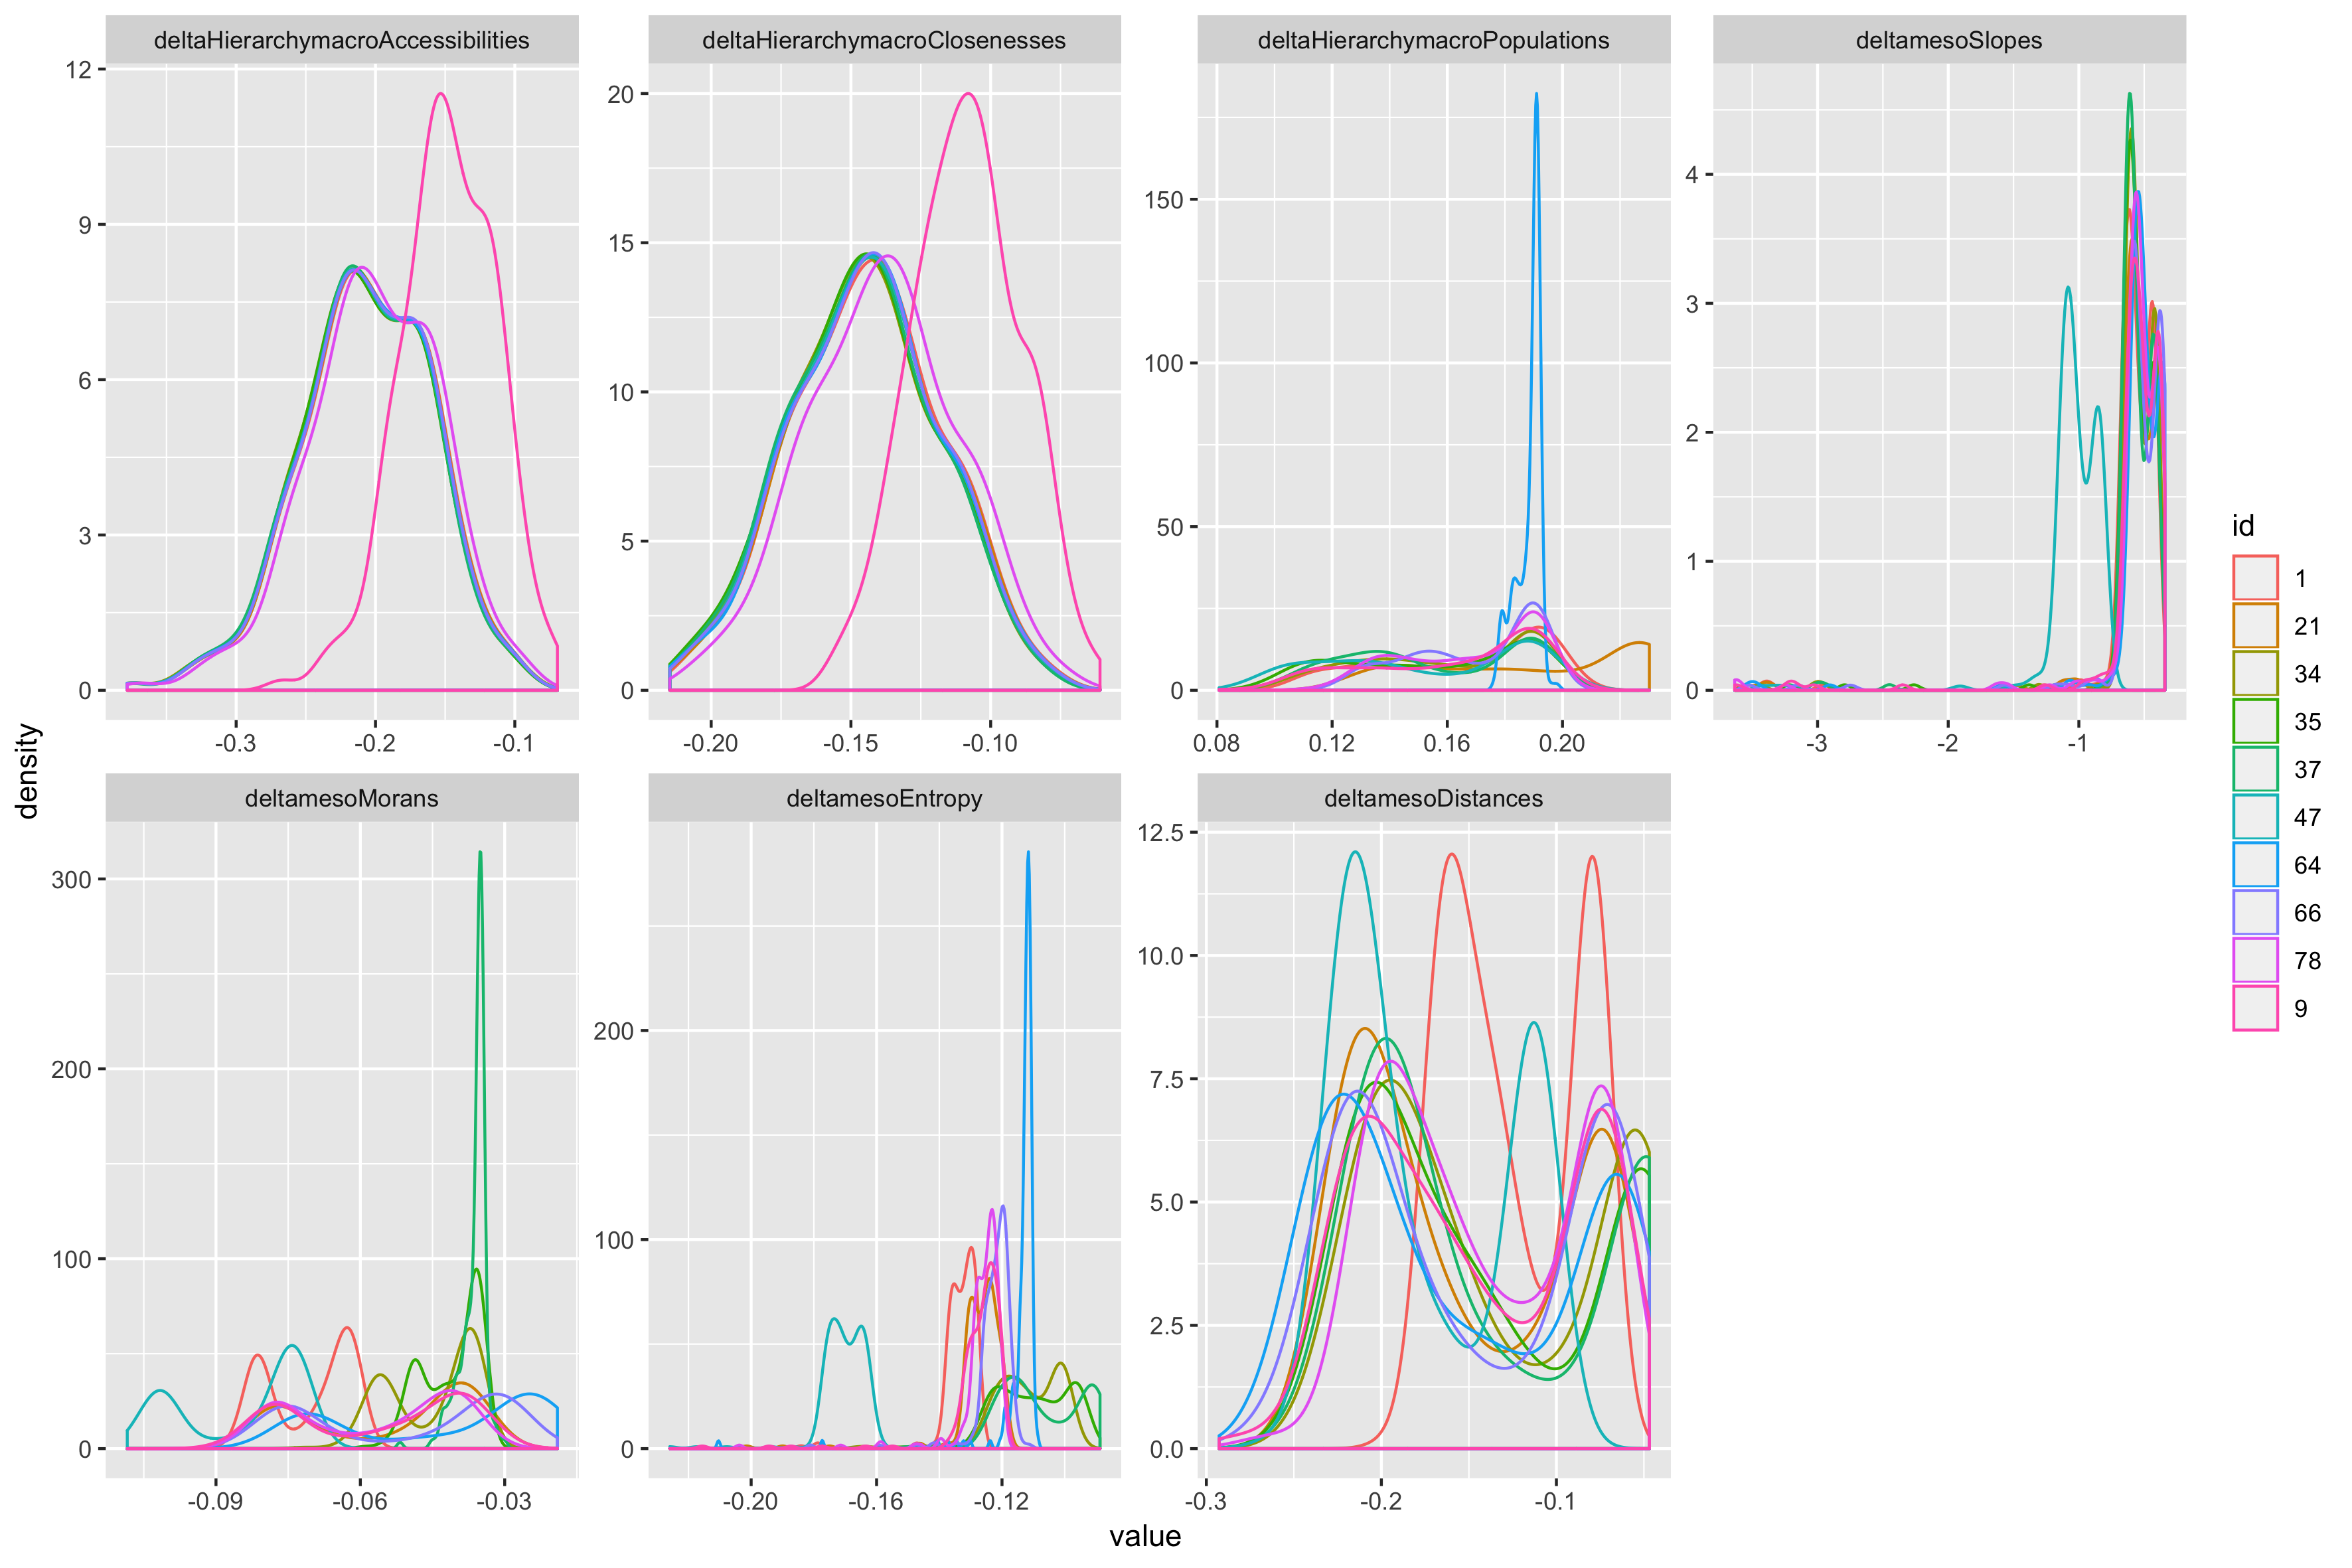
\includegraphics[width=0.8\textwidth]{figures/allindics_hist.png}
\end{center}

\textit{For all indicators, median sharpe ratios computing for a parameter point across repetitions are all larger than 1.6}

}


\sframe{Model exploration}{

% First results show a strong impact of the strong meso-macro coupling, such as for example a qualitative inversion of the behavior as a function of interaction range of macroscopic indicators trajectories when switching from a ``transit-oriented development'' scenario (negative feedback of population growth on diffusion) to a ``sprawl'' scenario (positive feedback). Similarly, mesoscopic urban form indicators are significantly influenced by the coupling process.
% ! abstract is wrong : say it !

\begin{center}
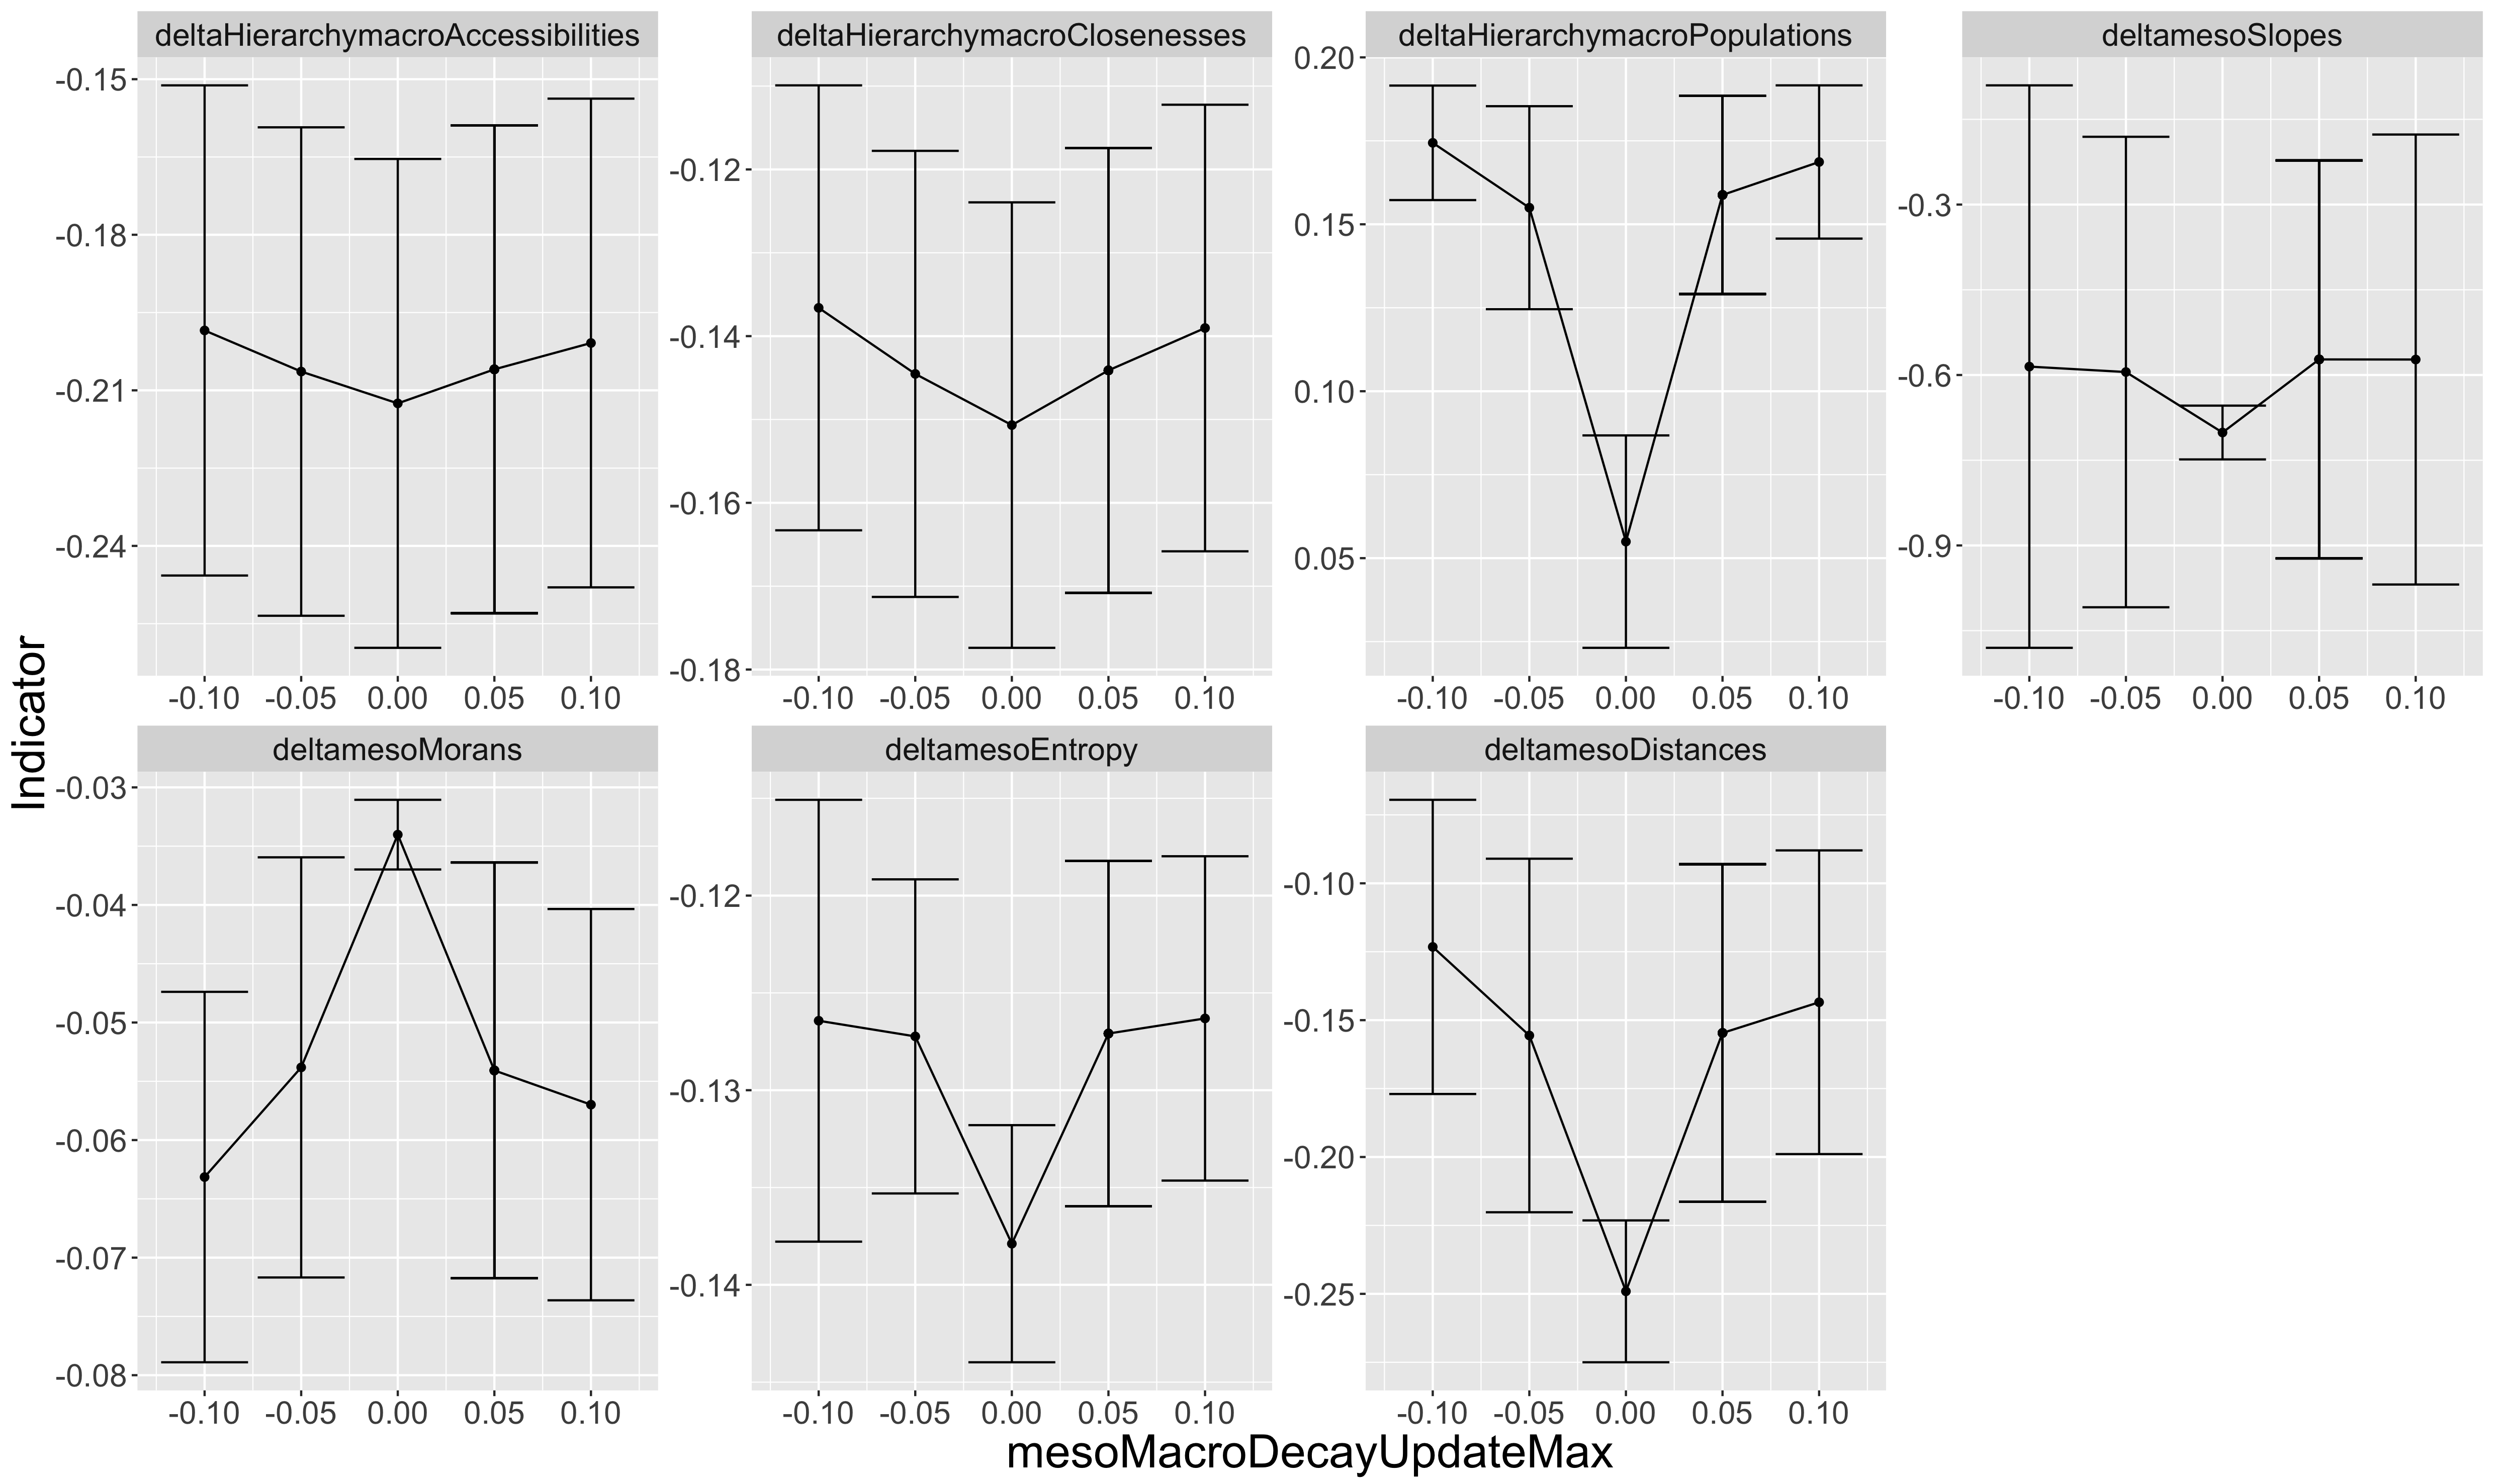
\includegraphics[width=\textwidth]{figures/onefactor_allindics_mesoMacroDecayUpdateMax_errorbars.png}
\end{center}

\footnotesize
\textit{U-shape behavior of both macroscopic and mesoscopic indicators as a function of $\delta d$}

}

\sframe{Model exploration}{

% what is interesting: that macro -> meso -> macro has indeed a role (or the other way around)

\begin{center}
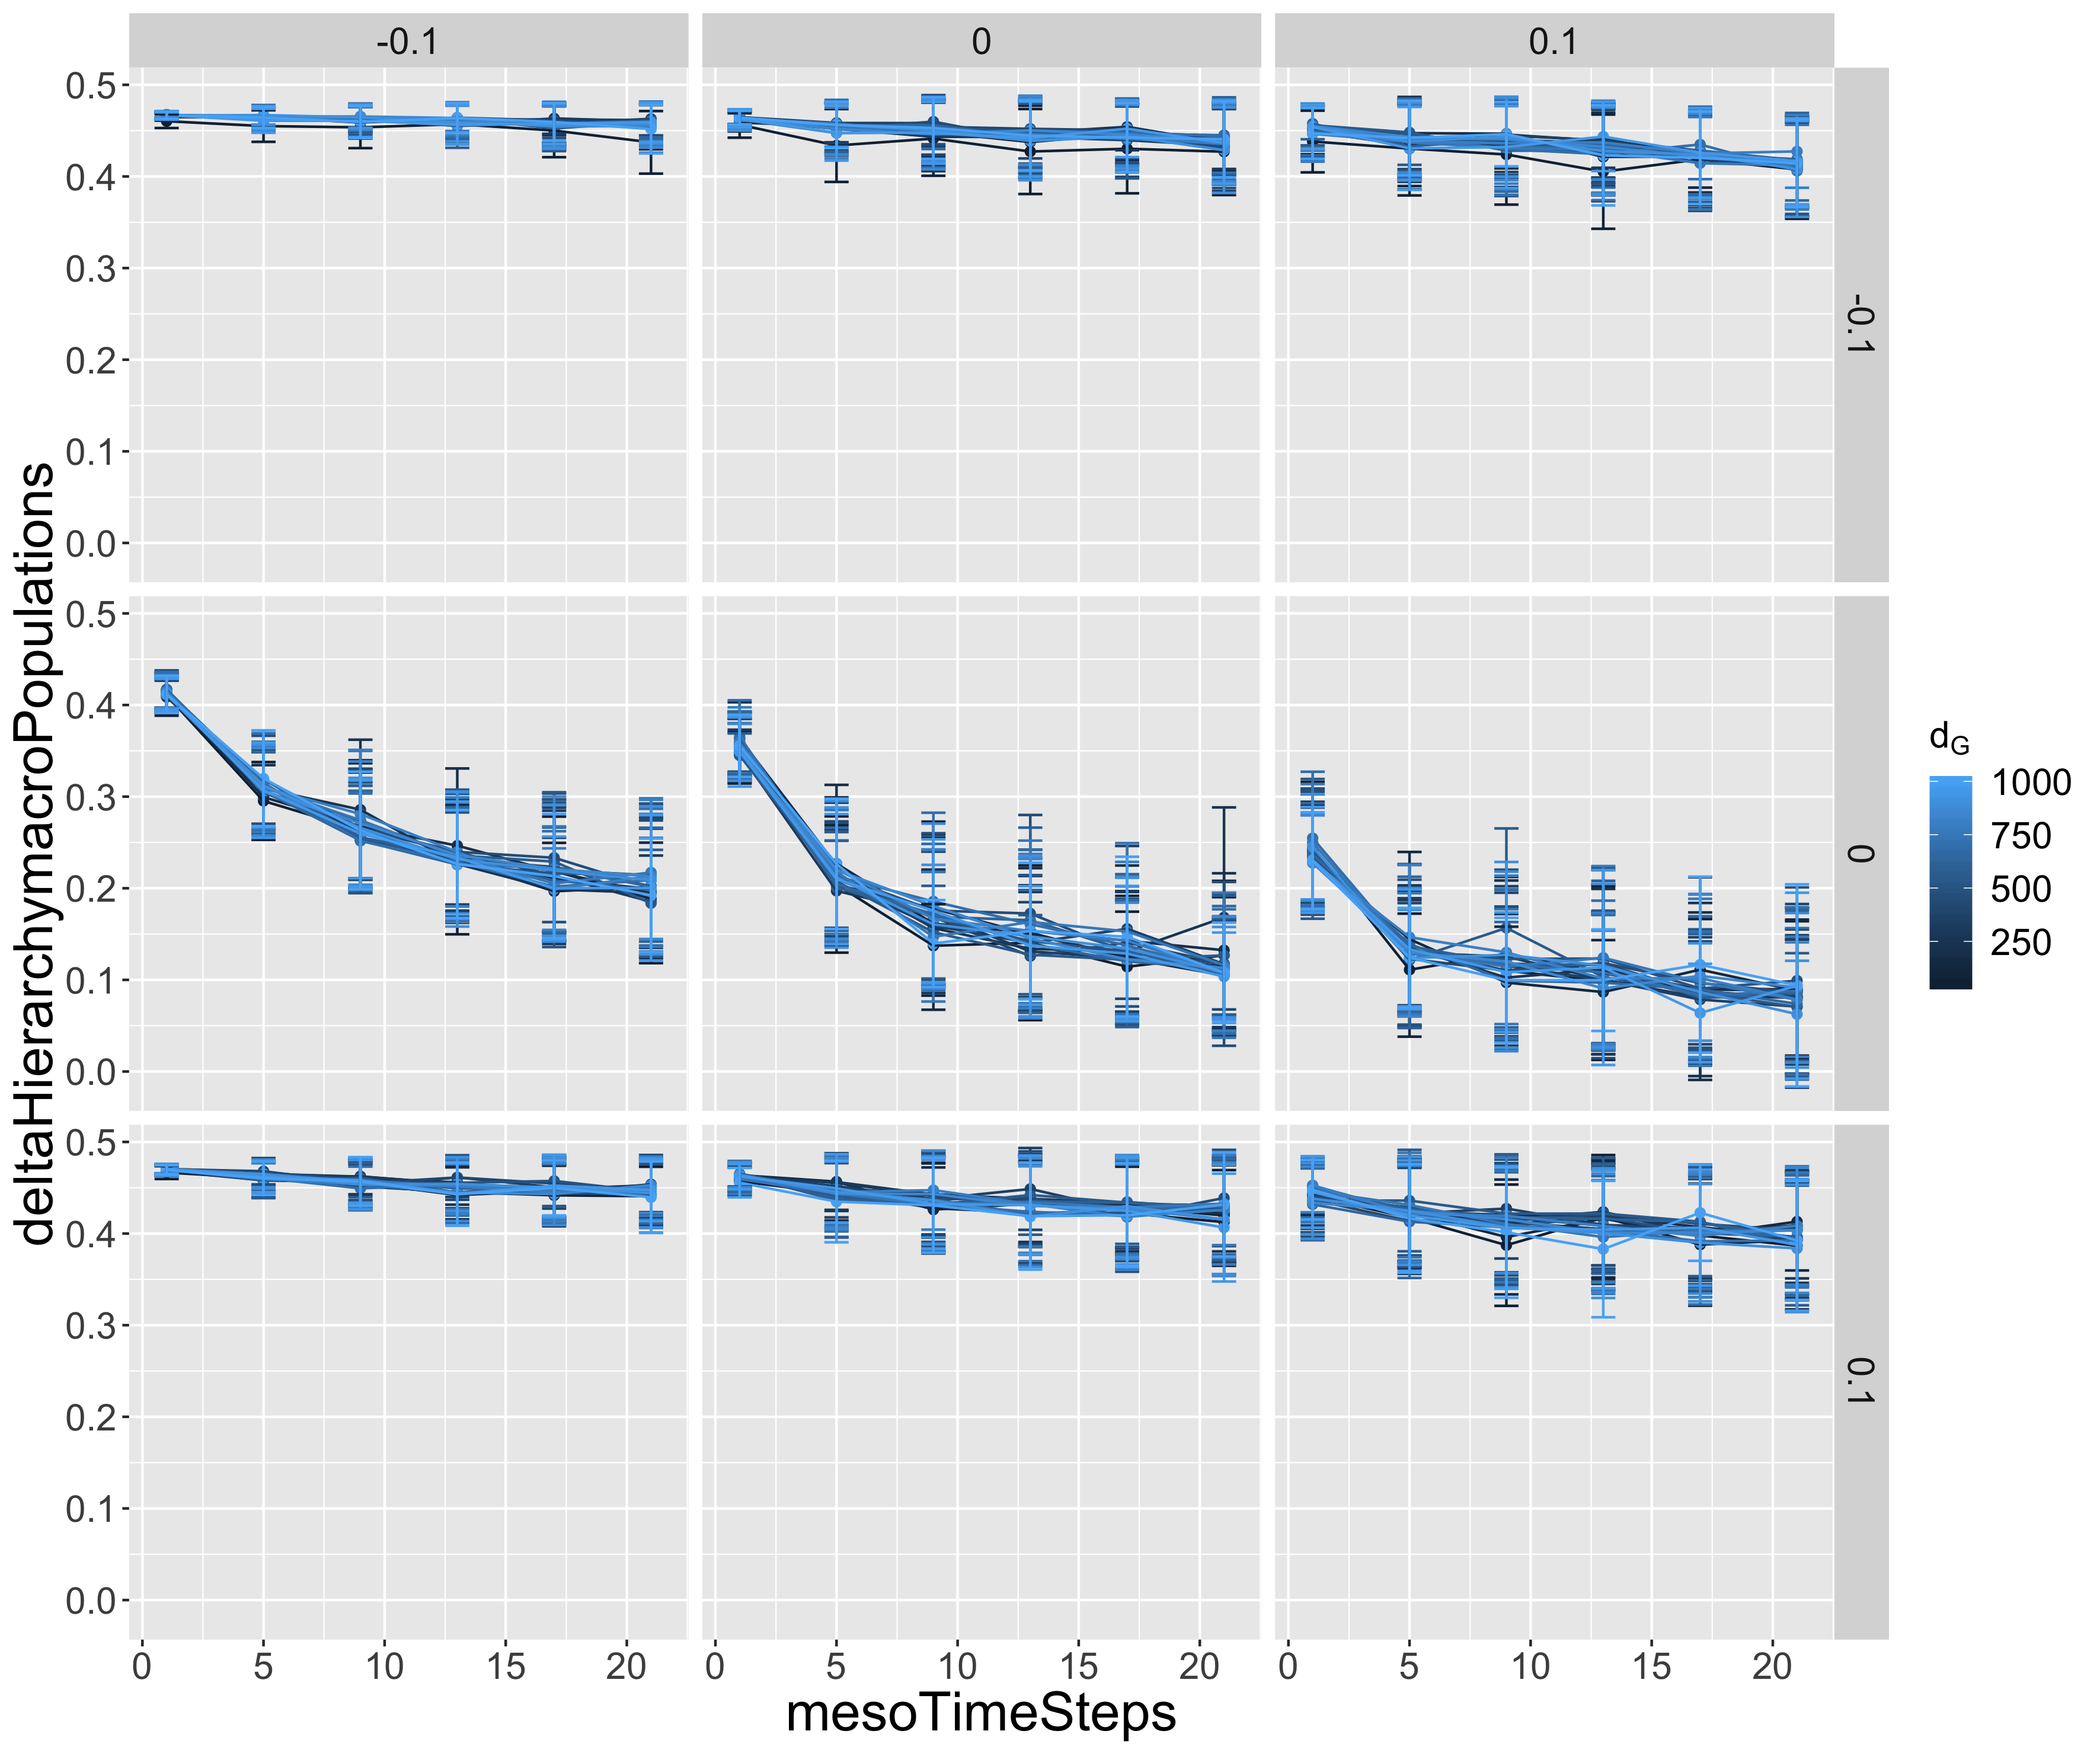
\includegraphics[height=0.75\textheight]{figures/deltaHierarchymacroPopulations-mesoTimeSteps_colorMacroInteractionDecay_facetmesoMacroDecayUpdateMax-macroMesoBetaUpdateMax.png}
\end{center}

%\footnotesize
\textit{Non-trivial influence of coupled feedbacks on the different scales}


}



\sframe{Impact of policy parameters}{

\begin{center}
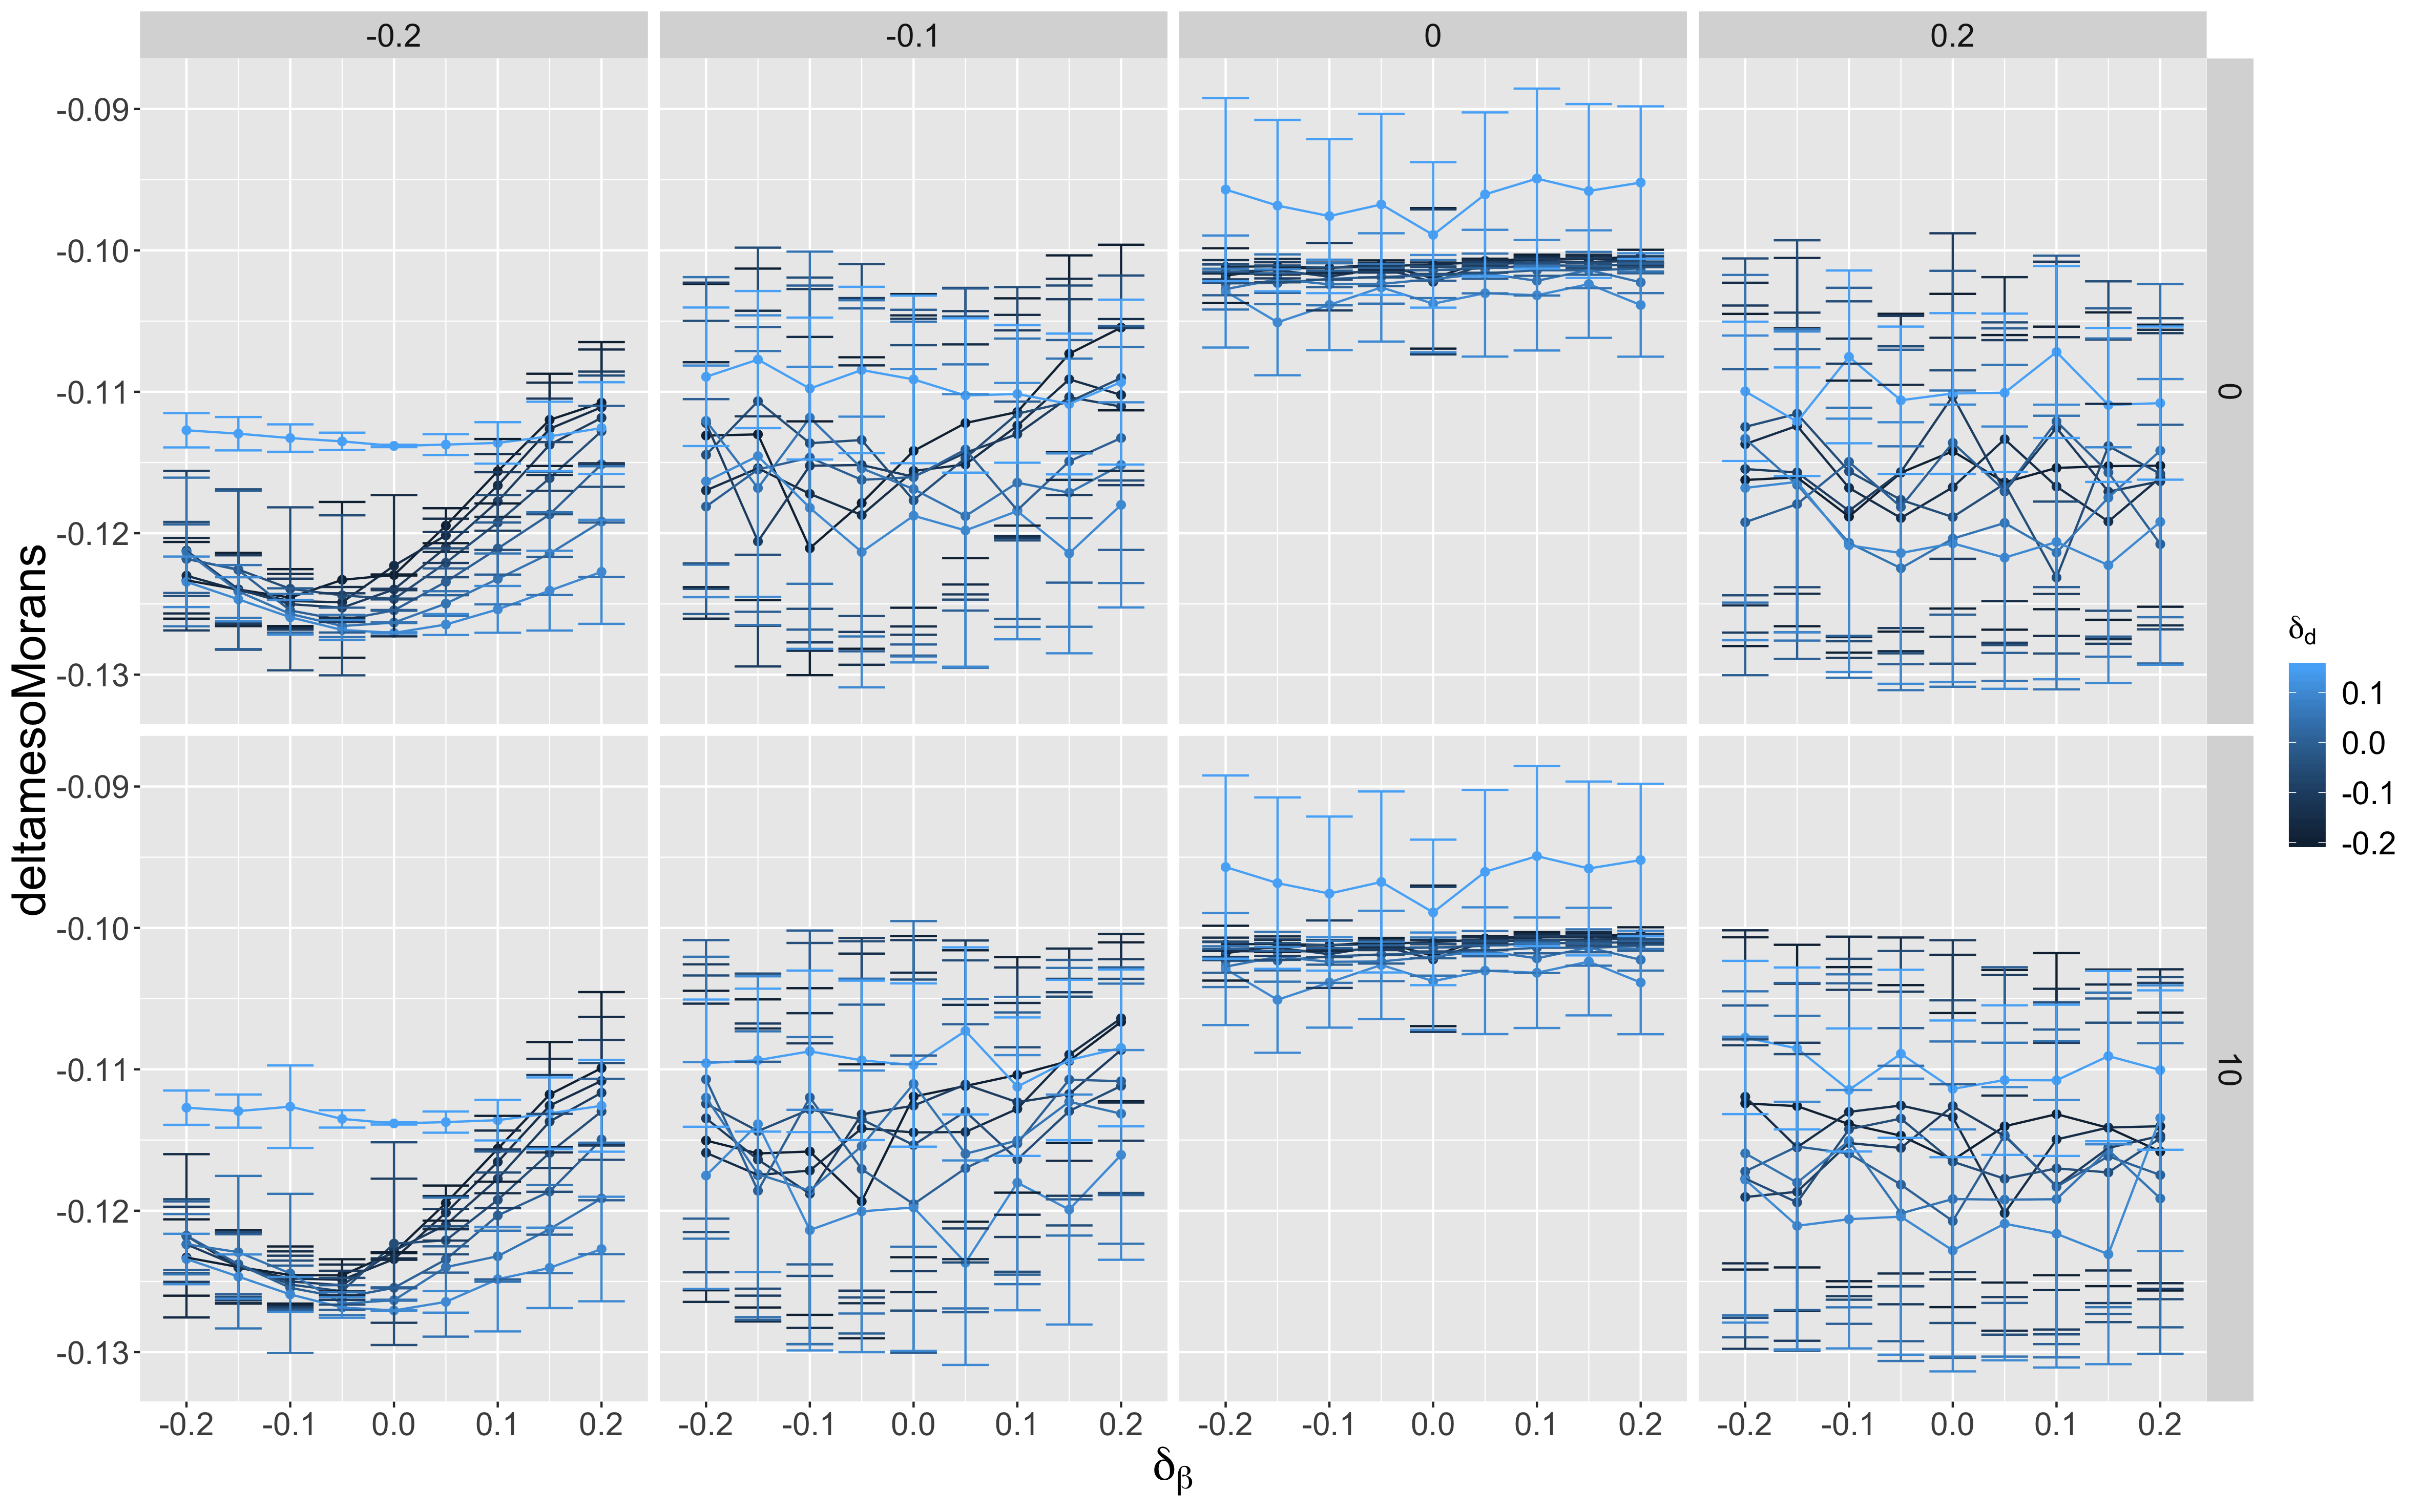
\includegraphics[height=0.7\textheight]{figures/deltamesoMorans-macroMesoAlphaUpdateMax_colormacroMesoBetaUpdateMax_facetmesoMacroCongestionCost-mesoMacroDecayUpdateMax_mesoBeta0_11.png}
\end{center}

\textit{Mesoscopic centralization appears at a $\delta \beta$ critical value for low $\delta \alpha$; influenced by upward feedback}

}

\sframe{Impact of policy parameters}{

\begin{center}
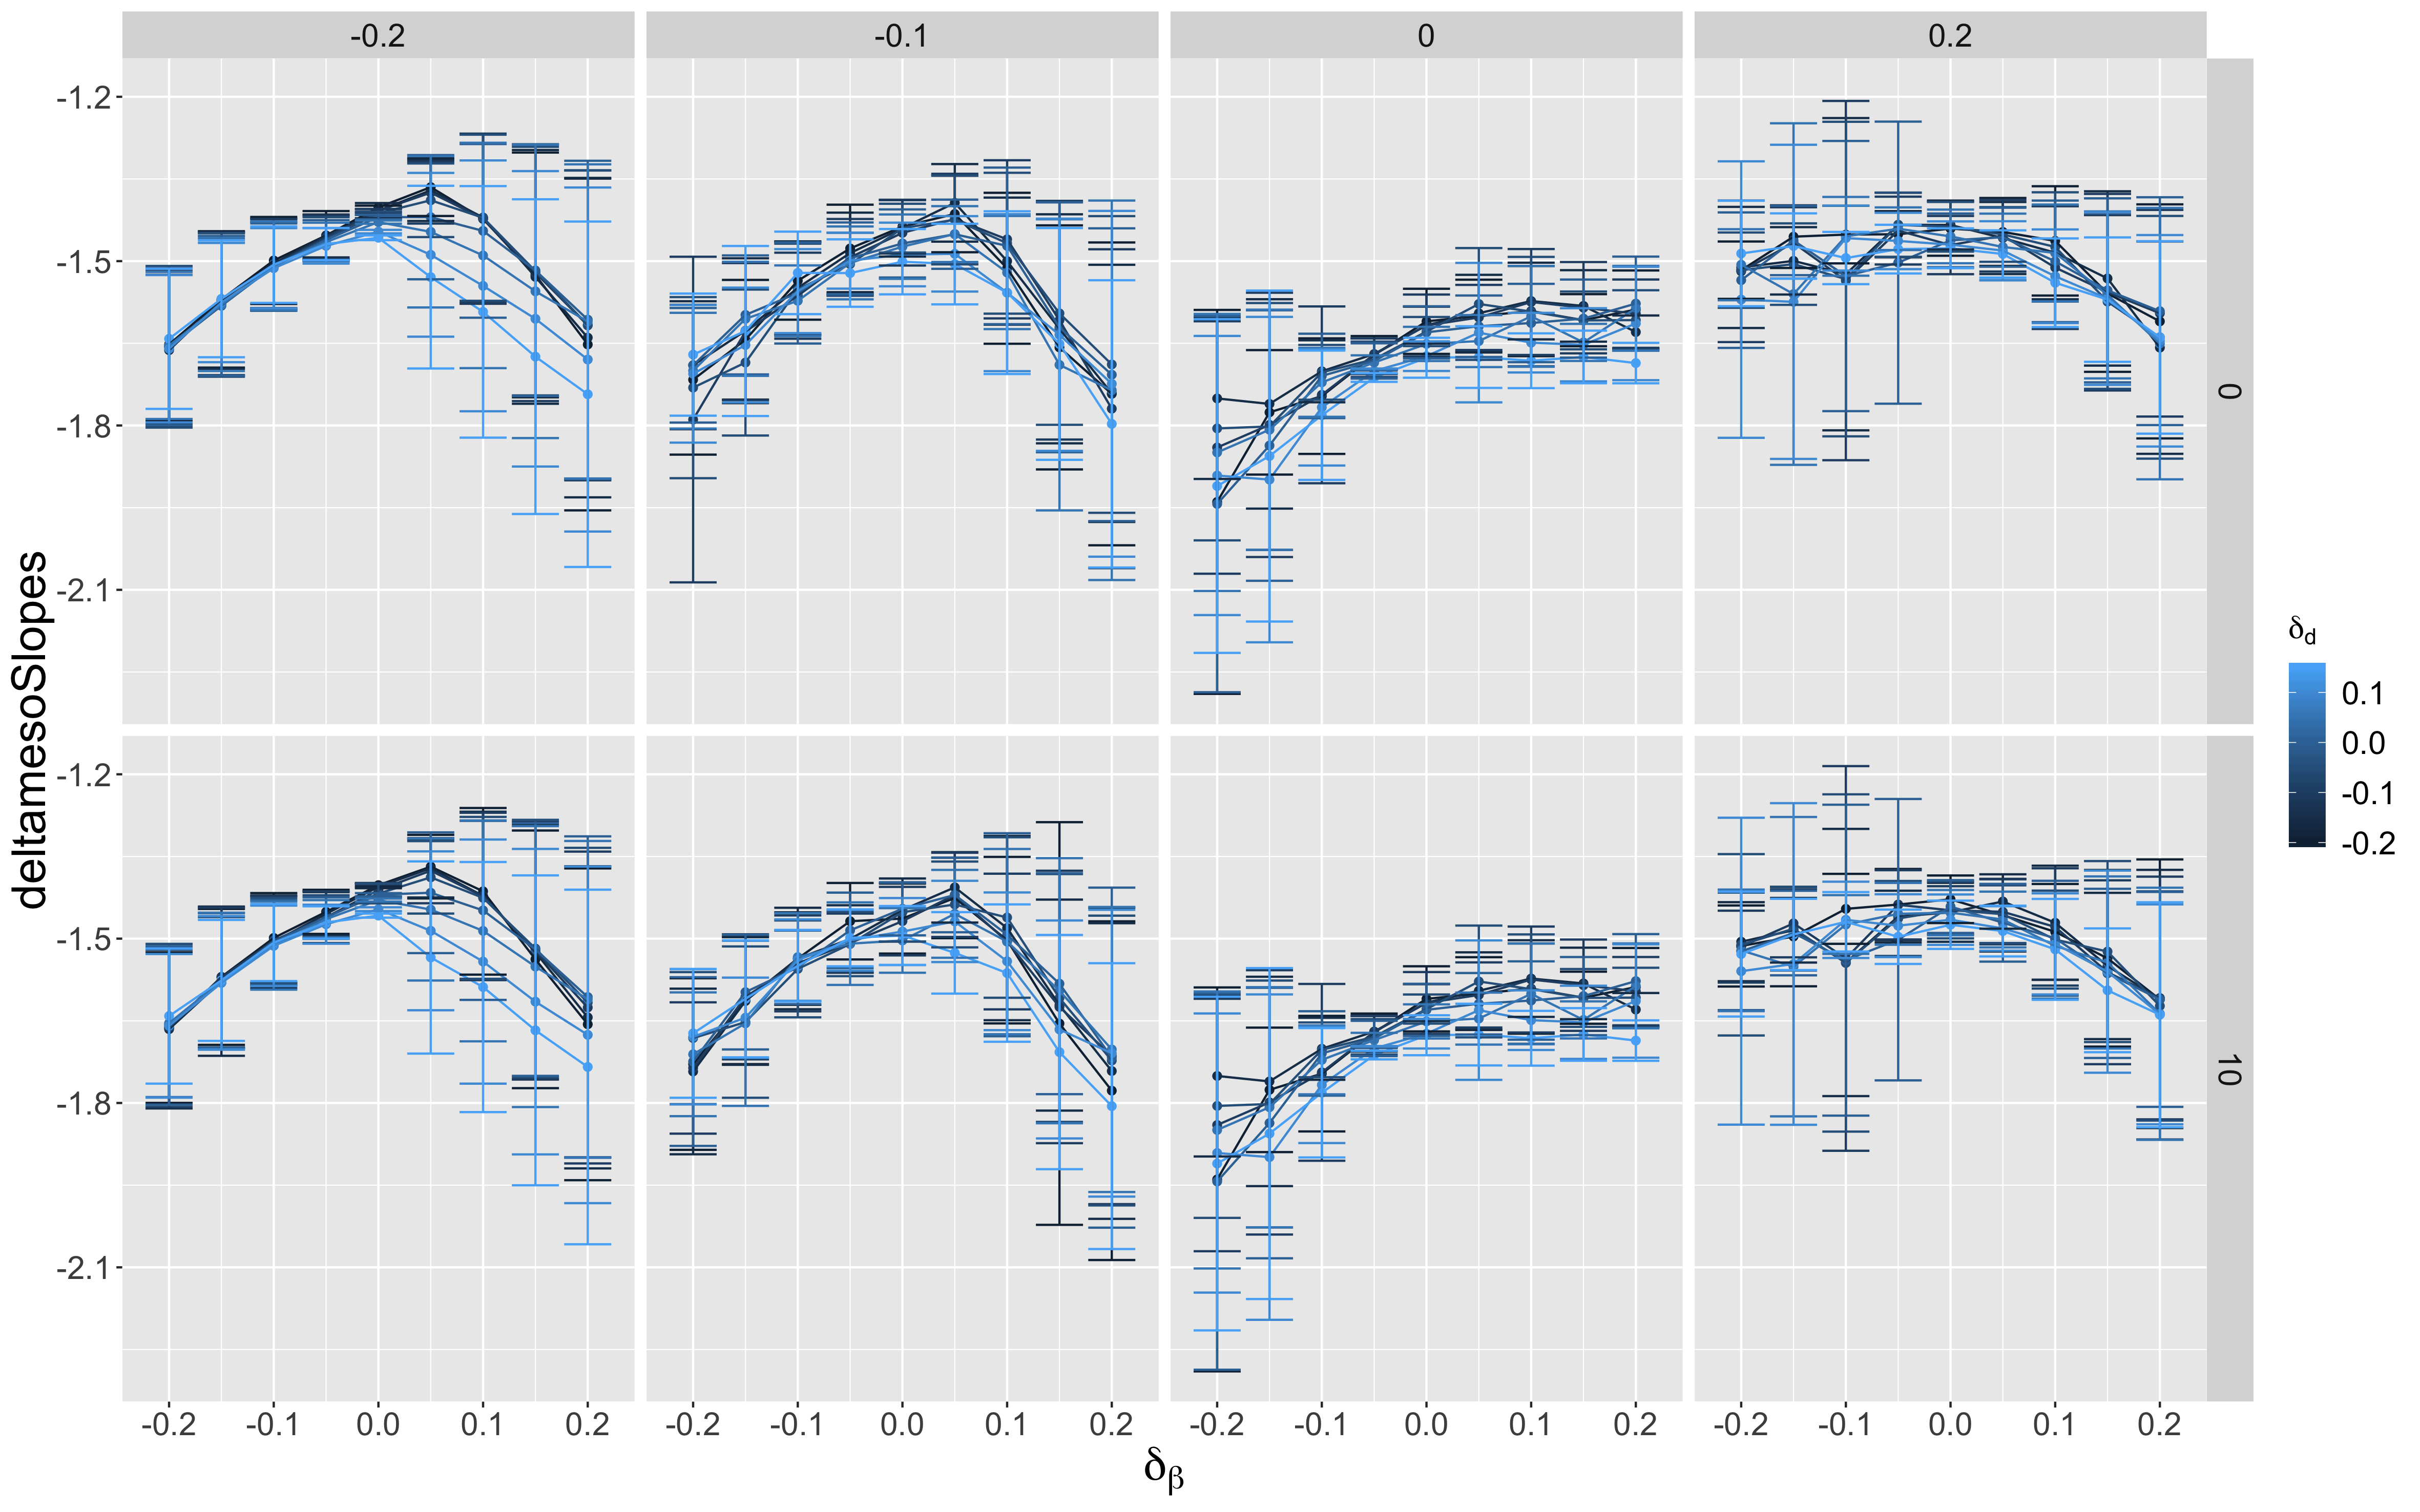
\includegraphics[height=0.7\textheight]{figures/deltamesoSlopes-macroMesoAlphaUpdateMax_colormacroMesoBetaUpdateMax_facetmesoMacroCongestionCost-mesoMacroDecayUpdateMax_mesoBeta0_11.png}
\end{center}

\textit{Mesoscopic hierarchy has a U-shape of $\delta \beta$ in negative $\delta \alpha$, but has a plateau for positive values} 
%$\rightarrow$ sprawl is needed in a sense

}




\sframe{Multiscale optimization}{

\begin{center}
	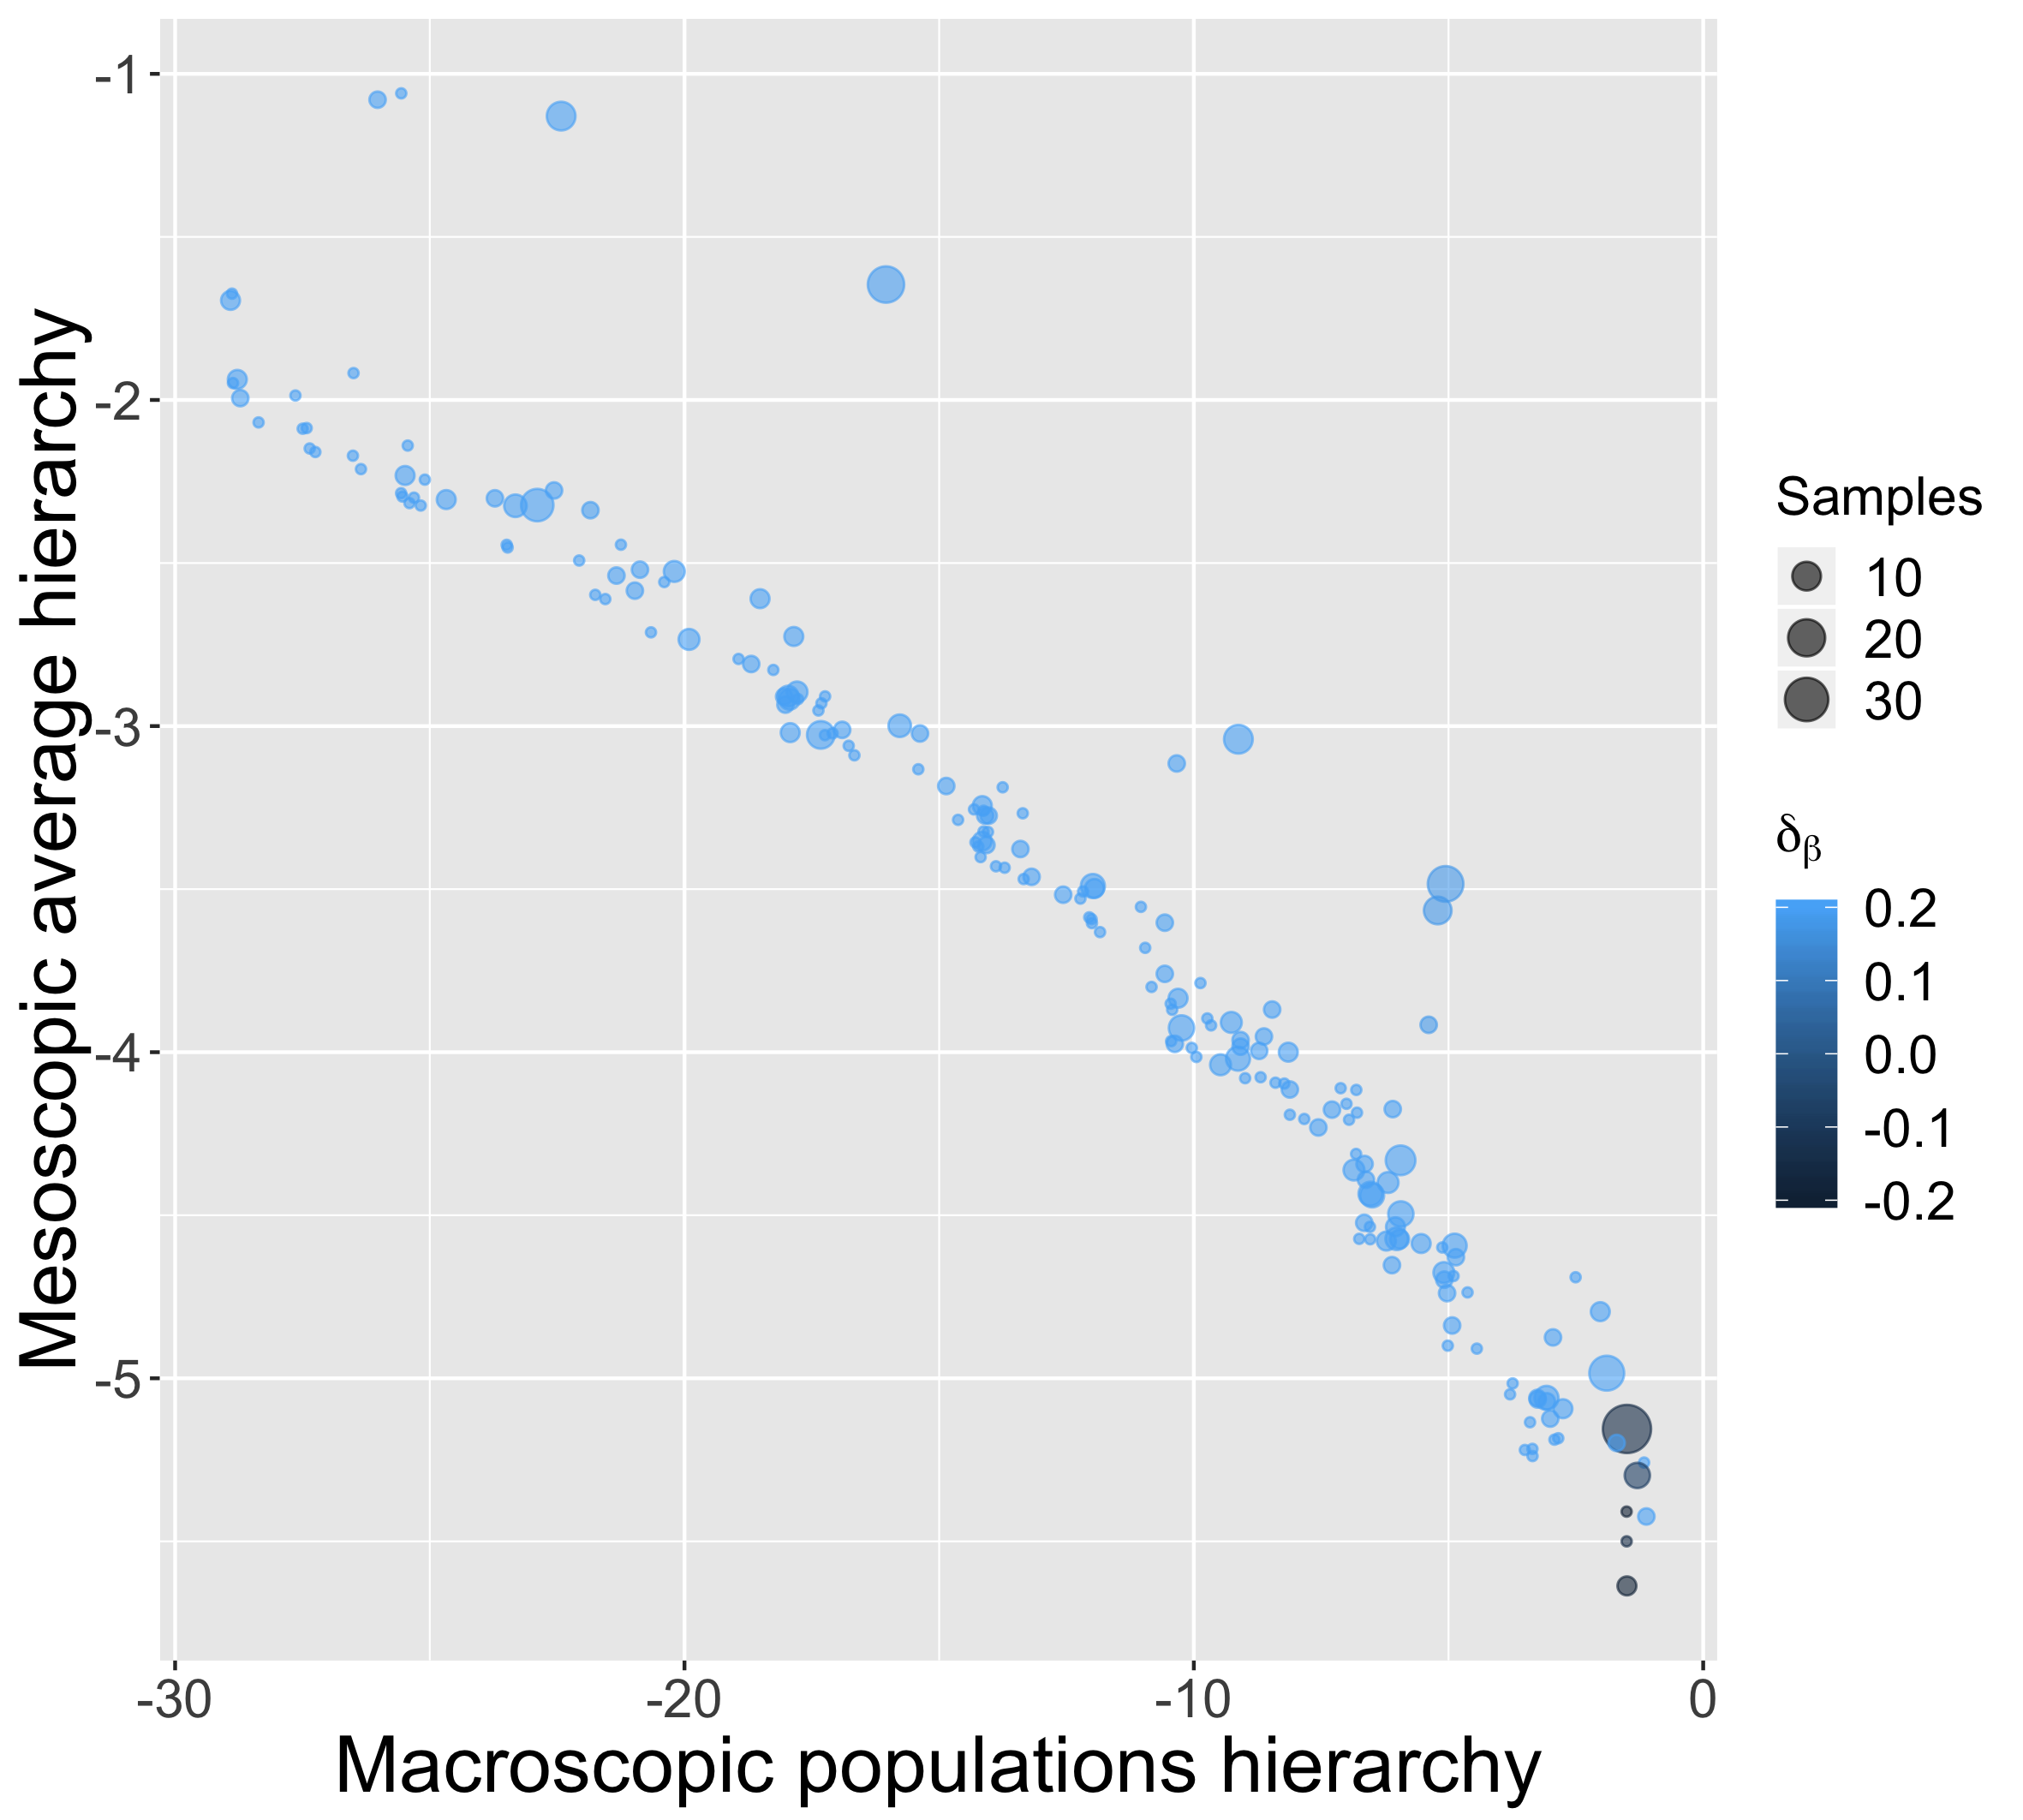
\includegraphics[width=0.8\textheight]{figures/pareto_macroHierarchy-mesoHierarchy.png}
\end{center}

\textit{Pareto front obtained with Genetic Algorithm optimization for two contradictory objective of macrosopic and mesoscopic hierarchies}

}




\section{Discussion}



\sframe{Discussion}{


%Further work will consist in more targeted simulation experiments, including specific exploration algorithms such as diversity search for model regimes \cite{reuillon2013openmole}, to test the model as a proof-of-concept of models for policies. Such a model can also be calibrated on real city systems and urban form trajectories, to extrapolate coupling parameters that would be difficult to obtain otherwise. 
\justify

\textbf{Theoretical and practical implications}

\medskip

$\rightarrow$ model effectively captures an interaction between downward and upward feedback: weak emergence \cite{bedau2002downward}

\medskip

$\rightarrow$ coupling ``simple three parameters models'' yield a complicated and complex simulation model: necessity of complexity and simulation models to understand urban complexity? 
% 'suggest in a way failure of reductionist empistemology (in the sense of a la Barthelemy) - at least for grabbing the multi-scalar nature of systems' (seems a tautology though

\medskip

$\rightarrow$ progressive integration towards models for policy?

\bigskip

\textbf{Developments}

$\rightarrow$ diversity search algorithm to find e.g. regimes with the strongest effect of feedback

\medskip

$\rightarrow$ parametrization on real systems; possibly calibration

(see \cite{raimbault2019ilus} forthcoming presentation at ILUS)


}




\sframe{Conclusion}{

% Our contribution is thus a first step towards multi-scalar simulation models for systems of cities.


$\rightarrow$ A first step towards \textit{strongly} multi-scalar models to capture urban complexity towards policy models

\medskip

$\rightarrow$ Towards integrative models and theories for urban systems \cite{raimbault2019methods}


\bigskip
\bigskip

\footnotesize

\textbf{Open repositories for}

\begin{itemize}
 \item Model: \texttt{https://github.com/JusteRaimbault/UrbanGrowth-model}
 \item Project: \texttt{https://github.com/JusteRaimbault/UrbanGrowth}
 \item Simulation data: \texttt{}% dataverse
\end{itemize}

\bigskip

\textbf{Acknowledgments}: thanks to the \textit{European Grid Infrastructure} for access to the infrastructure.


}



\sframe{Reserve slides}{

\centering

\Large

\textbf{Reserve Slides}

}




\sframe{Mesoscopic model}{


$\rightarrow$ Grid world with cell populations $\left(P_i\left(t\right)\right)_{1\leq i\leq N^2}$.

\bigskip

$\rightarrow$ At each time step:

\begin{enumerate}
\item Population growth with exogenous rate $N_G$, attributed independently to a cell following a preferential attachment of strength $\alpha$
%\begin{equation}
%\Pb{P_i(t+1)=P_i(t)+1|P(t+1)=P(t)+1}=\frac{(P_i(t)/P(t))^{\alpha}}{\sum(P_i(t)/P(t))^{\alpha}}
%\end{equation}
%The attribution being uniformly drawn if all population are equal to 0.
\item Population is diffused $n_d$ times with strength $\beta$
\end{enumerate}

\bigskip

$\rightarrow$ Stopping criterion: fixed maximal population $P_m$.

%To avoid bord effects such as reflecting diffusion waves, border cells diffuse their due proportion outside of the world, implying that the total population at time $t$ is strictly smaller than $N_G\cdot t$.

\bigskip

$\rightarrow$ Output measured by morphological indicators: Moran index, average distance, rank-size hierarchy, entropy.




}



\sframe{Model formalization}{


\textit{Macroscopic interactions}

\medskip

\begin{equation}
		P_i\left( t \textrm{ + } 1 \right) \textrm{ = } P_i\left(t\right) \left(1 \textrm{ + } \Delta t \cdot \left(g_i \textrm{ + } \frac{w_i}{N} \cdot \sum_j \frac{V_{ij}}{<V_{ij}>} \right) \right)
	\end{equation}
	
where the gravity interaction potential is given by 
	
\begin{equation}
		V_{ij} \textrm{ = } \left(\frac{P_i P_j}{(\sum_k p_k)^2}\right)^{\gamma_G} \cdot \exp \left(- \frac{d_{ij}}{d_i} \right)
\end{equation}

\medskip

Accessibility given by

\begin{equation}
	Z_i \textrm{ = } \sum_j \frac{P_j}{\sum_k P_k} \cdot \exp( - d_{ij} / d_i)
\end{equation}

}


\sframe{Model formalization}{

\begin{itemize}
	\item Mesoscopic growth rate
			    $N_G^{\left(i\right)} \left(t \textrm{ + } 1\right) = \Delta P_i / t_m$
	\item Sprawl parameter (population pressure)
		\begin{equation}
			\beta_i \left(t \textrm{ + } 1\right) \textrm{ = } \beta_i \left(t\right) \cdot \left(1 \textrm{ + } \delta\beta \cdot \frac{\Delta P_i (t)}{\max_k  \Delta P_k \left(t\right)}\right)
		\end{equation}
	\item Aggregation parameter (metropolization process)
	    \begin{equation}
			\alpha_i \left(t \textrm{ + } 1\right) \textrm{ = } \alpha_i \left(t\right) \cdot \left(1 \textrm{ + } \delta\alpha \cdot \frac{\Delta Z_i (t)}{\max_k  \Delta Z_k \left(t\right)}\right)
		\end{equation}

\end{itemize}


}

\sframe{Model formalization}{

Congested flows within the mesoscopic zones:

\begin{equation}
		U_i \textrm{ = } \sum_{kl} \left( \frac{P_k P_l}{P^2} \cdot \frac{1}{d_{kl}} - \lambda \left(\frac{P_k P_l}{P^2} \cdot \frac{1}{d_{kl}}\right)^2 \right)
\end{equation}
	
\bigskip
	
Update the macroscopic interaction distance accordingly

\begin{equation}
	d_i \left(t \textrm{ + } 1\right) \textrm{ = } d_i \left(t\right) \left( 1 \textrm{ + } \delta d \cdot \frac{U_i}{\max_k \left|U_k\right|} \right)
\end{equation}

}



\sframe{Morphological indicators}{

\begin{enumerate}
\item Rank-size slope $\gamma$, given by $\ln \left( P_{\tilde{i}}/P_0\right) \sim k + \gamma\cdot \ln \left(\tilde{i}/i_0\right)$ where $\tilde{i}$ are the indexes of the distribution sorted in decreasing order.
\item Entropy of the distribution:
\begin{equation}
\mathcal{E} = \sum_{i=1}^{M}\frac{P_i}{P}\cdot \ln{\frac{P_i}{P}}
\end{equation}
$\mathcal{E}=0$ means that all the population is in one cell whereas $\mathcal{E}=0$ means that the population is uniformly distributed.
\item Spatial-autocorrelation given by Moran index, with simple spatial weights given by $w_{ij} = 1/d_{ij}$
\[
I = M \cdot \frac{\sum_{i\neq j} w_{ij} \left(P_i - \bar{P}\right)\cdot\left(P_j - \bar{P}\right)}{\sum_{i\neq j} w_{ij} \sum_{i}{\left( P_i - \bar{P}\right)}^2}
\]
\item Mean distance between individuals
\[
\bar{d} = \frac{1}{d_M}\cdot \sum_{i<j} \frac{P_i P_j}{P^2} \cdot d_{ij}
\]
where $d_M$ is a normalisation constant
\end{enumerate}



}




%%%%%%%%%%%%%%%%%%%%%
\begin{frame}[allowframebreaks]
\frametitle{References}
\bibliographystyle{apalike}
\bibliography{biblio}
\end{frame}
%%%%%%%%%%%%%%%%%%%%%%%%%%%%










\end{document}

